\documentclass[12pt]{article}
\usepackage{amsmath}
\usepackage[margin=1in]{geometry}
\usepackage{setspace}
\usepackage{graphicx}
\usepackage{wasysym}
\usepackage{float}
\usepackage [english]{babel}
\usepackage [autostyle, english = american]{csquotes}
\MakeOuterQuote{"}
\doublespacing

\graphicspath{{images/}{plots/}}

\author{Tyler Reisinger}
\title{Effect of Jupiter-sized Planet Interactions on Planetary Systems}
\date{}

\begin{document}

\begin{titlepage}
    \begin{center}
        \vspace*{1cm}
        
        \textbf{Effect of Strong Stellar Interactions on Planetary Systems and
            the Formation of Hot Jupiters}
        
        \vspace{1.5cm}
        
        \textbf{Tyler Reisinger}\\
        Under the guidance of Dr. Steve McMillan and Joseph Glaser
        
        \vfill
        
        Submitted in partial fulfillment of the requirements for the
        degree of Bachelor of Science in Physics
        
        \vspace{0.8cm}

        Department of Physics \\
        Drexel University \\
        Philadelphia, PA, United States\\
        8th of June, 2017 
    \end{center}
\end{titlepage}

\tableofcontents

\clearpage

\section{Abstract}

"Hot Jupiters" (HJs) are large planets that orbit very close to their host star. 
They appear to occur relatively frequently in the universe, with approximately 1\% 
of sun-like solar systems predicted to contain one (Brucalassi et al. 2016). 
However, the mechanism that causes these planets to have such extreme orbital parameters
is not fully understood. 
We aim to explore the role that star-planet and planet-planet gravitational interactions 
within a star cluster may have in producing Hot 
Jupiters. By using computational simulations of "typical" star clusters,
we will attempt to probe what happens over vast periods of time
in star clusters similar to those found within the Galaxy.
We will run detailed simulations of close stellar encounters within these clusters
and observe the resulting state of the systems after the stars have separated. Many
of these system are then computationally analyzed.
As a result of these simulations, 
we hope to observe the formation of Hot Jupiter-like orbits that
match observational data as well as determine how common an occurrence they are.
Additionally, we can observe what other damage might 
persist within the planetary orbits of the system that can be used as 
observational evidence for this formation scenario. Finally, we will
produce a collection of code which may be used in the future to perform similar
experiments.

\clearpage

\section{Introduction}

\subsection{Theory}

In the study of exoplanets, one interesting class of planets are the so-called "Hot Jupiters" -- planets with a mass near that of Jupiter 
that have orbits of very small radius around their host star, generally with little eccentricity.
Hot Jupiters are interesting as their orbits approach very close to the host star,
despite the fact that most Jupiter-mass planets are believed to form much farther
out -- in the accretion disk of the forming planetary system where gases 
and other diffuse material can aggregate to form a new planet. If we look at our own
solar system, we see that Jupiter orbits at around 5.2 Astronomical Units (AU) from the
sun, where one AU is the average orbital distance of the Earth. Indeed,
we see a very large gap between the orbits of the inner, small and rocky planets, and
the outer gas planets, of which Jupiter is the nearest. Jupiter is not an anomaly of
the universe, but rather many gas giants are seen in a similar orbit. %TODO: Verify me

The Hot Jupiters seen in the universe, however, have orbital 
radii of only fractions of an AU, potentially 
approaching their star closer than even Mercury in our own solar system. %TODO: Expand on planet formation theory.

Normal planet formation theorizes that young stars are surrounded by an "accretion disk"
of dust and gas that remains from the star formation process. Nearest the star, radiative
pressure and energy evaporates water and other gases, as well as pushing them outward. 
This means the concentration of frozen gases
is greater some 4 AU and farther from a sun-like star. It is in this region where most
gas planets are thought to form (Pollack et al. 1996).

However, in the case of Hot Jupiters, their orbit much closer to the star --  
beyond the accretion disk. 
Therefore, the formation mechanism of Hot Jupiters
must be somehow different from that of "average" Jupiter planets, such as the one in our
solar system.

The mode of formation for Hot Jupiters is not fully understood.
Despite this, and their rather exotic orbits, 
they appear to be somewhat common within the universe as observations and previous models place the occurrence of Hot Jupiters at around 1\% of all solar systems (Brucalassi et al. 2016).  

A reasonable hypothesis for the formation of these Hot Jupiters is that they are not formed in place, but rather form much like normal gas giant planets 
in a gas and dust accretion disk beyond the ice line. They then migrate to their final close orbit sometime later after their formation. 
In order for the Hot Jupiter to move into a close orbit after it is formed, some sort of interaction must occur to change the orbital parameters. 
Disk migration theory postulates that the accretion of gases and 
solids during the planet's formation process can slowly alter the orbital 
parameters of the planet,
pushing the planet inward towards the star (Pollack et al. 1996).
This is thus a potential mechanism for the creation of these Hot Jupiters, but is not the end of the story.

New stars in the Galaxy generally form not as isolated individuals but rather in groups of stars
that then gravitationally interact to form a cluster.
Within one of these star clusters, there are times when two stellar systems approach very close
to one another. Depending on the closeness of the approach, the effects of such
an interaction may very. An encounter at a distance of a few hundred AU will likely disturb the trajectory
of the two stars in the short term, but is unlikely to have other significant effects. However,
if the two stars come close enough that the approaching star's gravitational attraction
overwhelms that of the host star, the planets around each star may have their orbits
highly disturbed. In this case, more distantly orbiting planets, such as the gas giants,
have a greater chance of being disturbed than the inner planets, as the two 
interacting stars do not need to get as close to affect the planetary orbits.

This gravitational "push" could also have many effects on the unlucky planets caught in the
middle. One likely outcome is that the planet's orbit is made more eccentric but otherwise
mostly unchanged. Additionally, the planet could be ejected from the planetary system,
or be captured by the approaching star -- orbiting it instead of the original host star
after the encounter is complete. A third possibility is that a Jupiter-like planet
from the outer solar system is thrown into an eccentric 
orbit that approaches much closer to the
star. In such a case, the orbit right after the interaction should have a highly
eccentric orbit, even if it passes close to the host star. 

Observed Hot Jupiter tend to have a rather circular orbit; in order for these stellar 
encounters to account for the observations, some process must make the orbits 
less eccentric. Since the Hot Jupiters are, by definition, close to the star and
also, due to their eccentricity, likely pass somewhat close to the inner planets of the
system (Earth in this case), tidal interactions may play a significant role in the
long-term dynamics of the system. Tidal effects can be numerous, but one common feature
is a slow "circularization", or decrease in eccentricity of the planet. This effect
plays out in megayear scales, and so is a long term change when compared to close stellar
encounters. (Rasiom et al. 1996)

Additionally, the inward movement of the larger gas planet could affect other
inner planets of the solar system during its transit. This can
cause the inner planet orbits to become more eccentric and could move
these planets closer or farther from the star depending on the details of the
interaction, or even eject them out of the system. Should this occur,
then another "pair" planet could be formed in the same system which has its orbit
disturbed by the migration of the gas giant rather than from the stellar encounter. 
This "pair" planet 
would likely also end up with an eccentric orbit like the outer planet. Pair planet formation would leave
a second long-term impact on the system, which may provide additional observational
evidence for this kind of migration having taken place.

Such an interaction also holds importance for the fate of Earth-like planets.
A planet formerly in the habitable zone of a star could be knocked into a far less
forgiving orbit, leading to likely fatal effects on life. Additionally, a
large planet in an eccentric orbit that passes within the inner planetary orbits,
even if it does not perturb these planets right away, might cause later chance
encounters between the planets that lead to orbital changes.

We will focus on the star cluster interactions and their potential to 
cause structural changes to the planetary systems involved. Using computer simulation,
we are able to probe the gravitational dynamics of these star system 
interactions over several thousand years of physical time 
in time scales much more accommodating to human lifespan. We will simulate
a large number of these interactions, building up a database of information about
the initial and final states of the systems. Using this data, we perform large
scale analyses, finding potential Hot Jupiter formation events, as well as other
significant perturbations to the planetary orbits.

By having a large database of encounter information, we also look for commonalities
and frequencies of the destructive events encountered. 

\subsection{Orbital Elements}

    An important set of information for analyzing the behavior of the stellar and
    planetary dynamics are the orbital elements that mathematically 
    characterize the motion of the planet relative to the host star. 
    For our purposes, we are most interested in the eccentricity $e$ and the
    semimajor axis $a$. The eccentricity describes how "long" the orbit is, $e=0$
    is a perfectly circular orbit whereas $0<e<1$ are elliptical orbits of increasingly
    oblong shape. Eccentricities $e>1$ define hyperbolic orbits where bodies are no longer
    gravitationally bound. Additionally, these two pieces of information allow us to 
    compute the closest and farthest points of a bound orbit by two simple relations.

    The pericenter or closest distance is:
    \begin{equation}
        r_{per} = (1 - e) a
    \end{equation}
    Whereas the apocenter or farthest distance is:
    \begin{equation}
        r_{apo} = (1 + e) a
    \end{equation}

    The pericenter particularly will allow us to characterize orbit migration where a
    planet moves closer or farther from the host star.

\section{Methods}

    \subsection{Infrastructure}

    Our approach was entirely computational in nature. We developed a collection of tools
    and utilities utilizing the popular Python programming language and making use
    of the AMUSE (Astrophysical Multipurpose Software Environment) library \footnote{The AMUSE library can be found at http://www.amusecode.org/. See references [5]-[8]}. 

    AMUSE provides the underlying gravitational simulation methods, with many different
    integrators and utilities for different needs. With AMUSE, we were able to 
    setup our problem and tell AMUSE to return to our code for encounter events and
    let AMUSE handle the rest. Additionally, AMUSE provides these features using high
    performance C++ and Fortran kernels, allowing us to focus on functionality without
    worry about the gravitational simulation details.

    N-body gravitational simulations with high accuracy and over long time scales require
    a significant amount of computationally expensive numerical integration of the 
    forces involved in the experiment. In order to exploit the parallel nature of 
    the simulations, our code was run mostly on the Draco computer 
    cluster at Drexel University. This cluster provides 24 connected nodes, each containing
    12 CPU cores as well as 4-6 GPUs. Utilizing this cluster, we were able to run many simulations in parallel.

    \subsection{Simulation}

    \subsubsection{Overview}

    The code has three logical phases forming a "pipeline" of data flow. 
    The first phase is to run simulations of typical
    star clusters and to record all "close encounters" between stars in the cluster.
    At this stage, there are no planets around the stars, but rather we will use the
    parameters of the close encounters to run more detailed simulations in isolation
    later.

    The second phase is running detailed simulations on the "close encounters". 
    A pair of interacting stars
    is placed into the simulation with the same dynamic parameters as in the cluster,
    and planets are added around each. A much shorter gravitational simulation is then
    run, allowing the systems to approach, interact and later separate. The final
    states of the two systems are recorded for the next phase.

    The final phase is to analyze the data generated from the previous simulations.
    Many simulations are run in order to develop a diverse profile of interactions.
    At this stage, we look for interesting encounters and related patterns, 
    what sorts of effects are most common,
    and the approximate frequency of certain outcomes. From here, the results can
    be used to verify the validity of the simulations with observation and to make
    predictions about these events in the universe.

    \subsubsection{Cluster N-Body Simulation}

    The N-Body simulation code is the first phase of the pipeline. In the
    universe, the dynamics of the star cluster and the dynamics of the
    interactions of planets around the containing stars are, of course, happening
    simultaneously. However, the dynamics of stars in a cluster are changing much
    more slowly than those of the planets because of the much larger distances
    involved. While a planet can fully rotate about a star in less than a year,
    only a handful of stars pass close to one another in a megayear. Accurately
    simulating planets around stars within a star cluster would require
    far more computation time, and most of this would be wasted simulating
    planets normally orbiting their host star far away from any other stars.

    The gravitational effects of an external star on a planet's orbit only
    causes noticeable orbital effects if the star comes within a few times the
    planet's orbital semimajor axis. This means that a Jupiter-like planet with an orbit around
    5 AU would only potentially be perturbed by a star that comes within 
    approximately 30 AU of the host star. Indeed, experimentally, we observe that
    encounters more distant than this leave almost no visible impact on the
    interacting systems. 

    The clusters created for this simulation are composed of one-thousand, two-thousand
    or four-thousand stars. For all three cases, the masses of all stars are set equally
    to $M = 1 M_{\astrosun}$. The simulations are run for a time directly proportional
    to the size, 250 Myr, 500 Myr and 1000 Myr respectively.  During the simulations, 
    any time two stars
    come close enough to strongly interact, the simulation is briefly halted so that
    the dynamical and orbital parameters can be recorded. The simulation is then
    resumed and this process repeats. At the end, a file is generated with
    all close encounters observed during the simulation, as well as the initial
    cluster bodies and information about the simulation itself.

    A "close encounter" as defined by this part of the code is when two stars
    come close enough to have a strong encounter between them. AMUSE decides
    this distance itself and notifies the simulation when this occurs. For planetary
    effects, we are generally uninterested in the majority of these encounters, however
    we choose to record all of these encounters for later filtering based on the
    planets being studied.

    The clusters generated for the simulation are uniquely created each time at the
    beginning of the simulation using a pseudo-random number generator. 
    The star properties are sampled from a standard statistical model for globular
    clusters called a
    %TODO: Reference
    King Model, with a fixed parameter $W_0=3.0$ (King, 1966).
    All stars added to the cluster are given a fixed mass $M=M_{\astrosun}$ and do not
    include any binary star systems.     

    \begin{figure}[H]
        \centering
        \caption{Two 2000-star clusters generated and simulated. The left plot
            shows the clusters at the start of the simulation. The right plot shows
            the same two clusters after 500 Myr of simulation time.}
        \begin{tabular}{cc}
            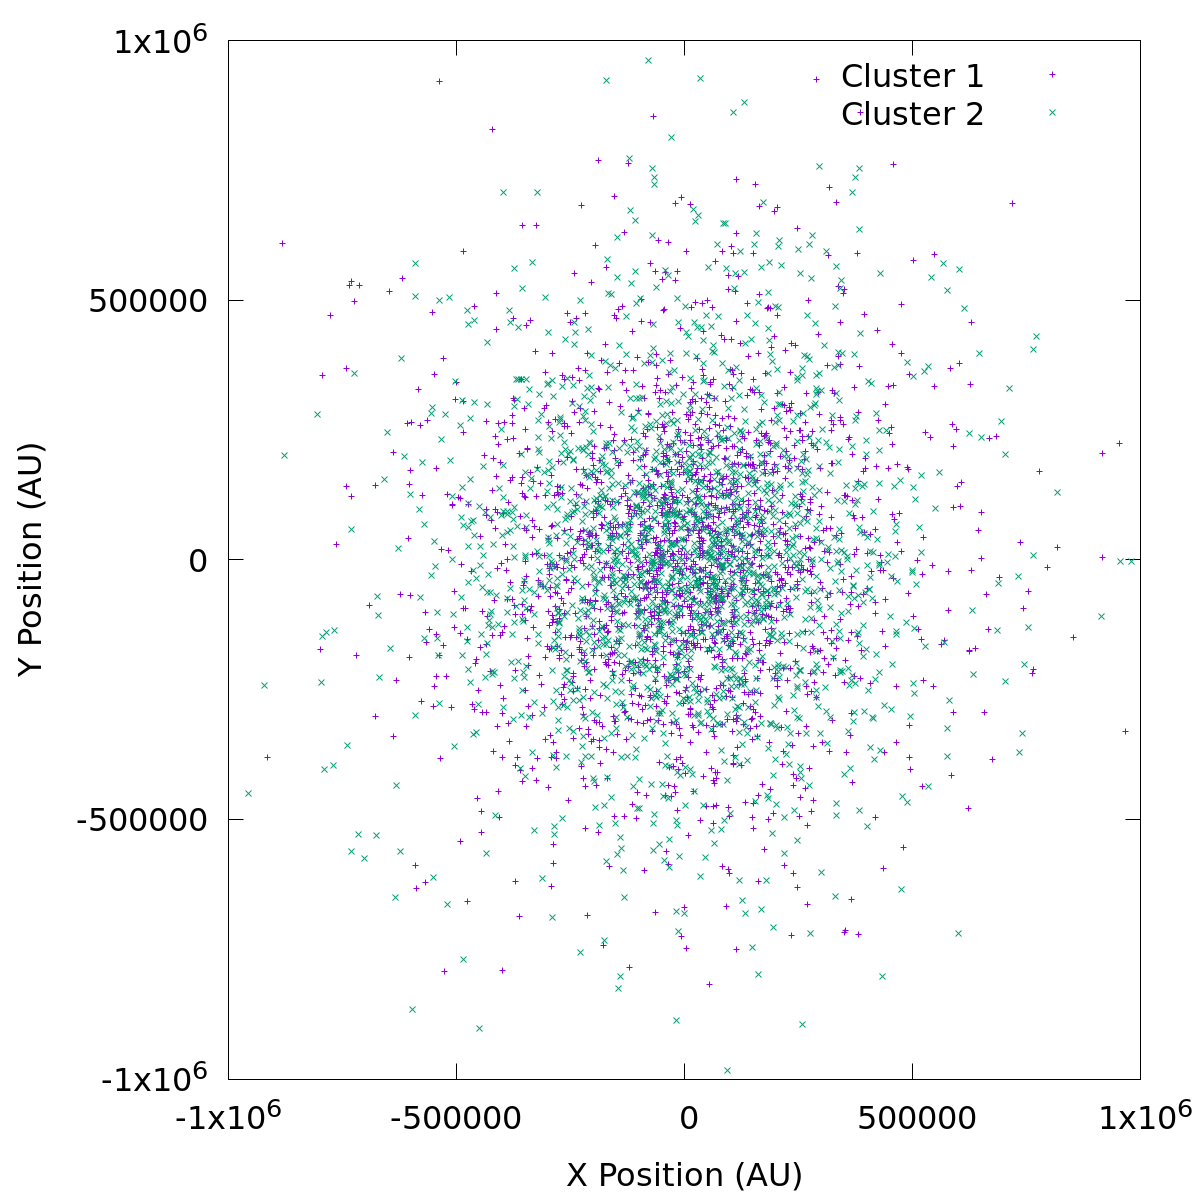
\includegraphics[width=3.0in]{clusters_superimposed_n_2000} &
            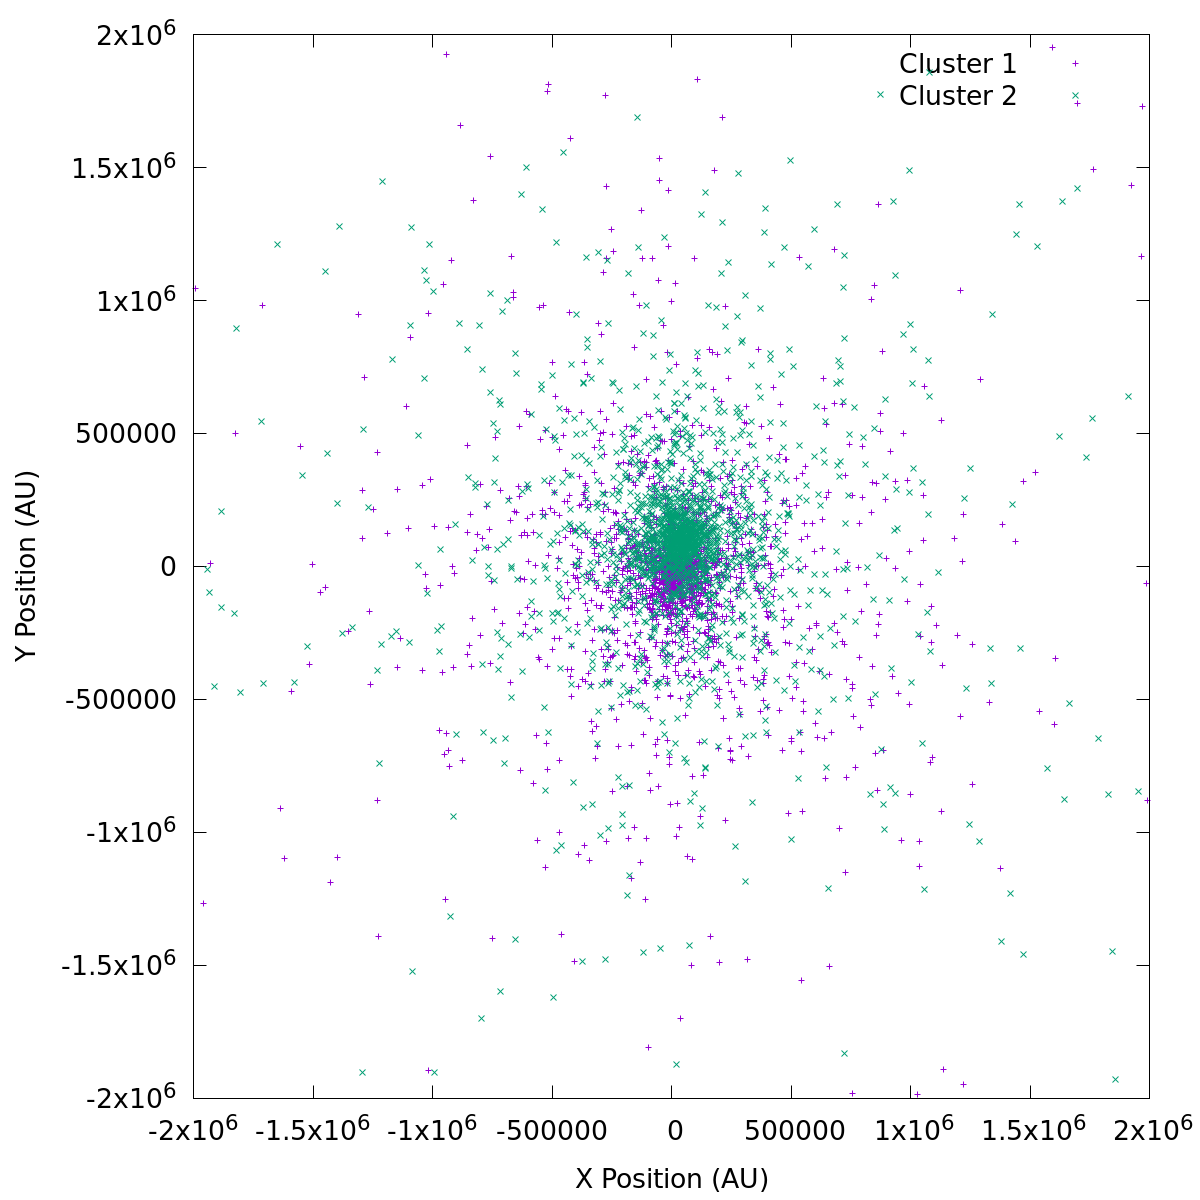
\includegraphics[width=3.0in]{clusters_superimposed_final_n_2000}
        \end{tabular}
    \end{figure}

    Each 100 megayears of simulation time for one of these clusters yields a
    few hundred encounters on average. The close encounters given to us by 
    AMUSE are based on the distance of the two stars at the time in the simulation
    when the two stars first get close enough to interact, around 400 AU.
    Since we are interested in planetary effects, only events where the stars
    then approach very near one another are interesting to us. In order to
    ignore more distant events in the future without having to run an expensive 
    planetary simulation for each, we compute the orbital elements of the two
    interacting stars, and use this with equation 1 to compute the approximate
    distance of closest approach. The closest approach distance, as well as 
    the orbital elements, are saved along with the encounter data for the later
    stages to use.

    Each of the three cluster sizes are simulated for the same total number of years.
    For the smallest configuration, one-thousand stars simulated for 250 megayears, 
    800 total clusters were simulated. For the two larger configurations, 400 and 200
    clusters were simulated respectively. All cluster simulations results are systematically 
    saved independently with information about the status and parameters of the run.
    This allows for taking subsets or samples of the data in the next stage, while still
    being easy to use all the results at once.

    The cluster simulations in this step require a considerable amount of clock time to perform,
    and the time required tends to increase by a factor of four for each doubling of the
    number of stars and simulation time. The 4000-star clusters each required around 60 to 120 minutes
    to perform. Even running up to twenty clusters at once, it required a few days to 
    simulate all of the clusters.

    In figure \ref{fig:encounter_distance}, we see the spectrum of closest approach
    distances observed in all encounters within the 1000-star clusters. The
    distribution is biased slightly toward the more distant encounters, which
    are the least likely to cause planetary effects. In this sample of data, there are
    57,351 total encounters with a closest approach distance under than 30 AU, 
    out of 1,831,075 total encounters. 
    This is just over 3\% of total encounters recorded. %Talk about Neptune

    \begin{figure}[H]
        \centering
        \caption{Closest approach of all recorded encounters in 800 1000-star cluster 
            simulations and 200 4000-star clusters. The larger clusters have more close
            encounters than the small ones.
            For Jupiter-Earth simulations, we are primarily interested in 
            those below 30 AU. 
        }
        \label{fig:encounter_distance}
        \begin{tabular}{cc}
            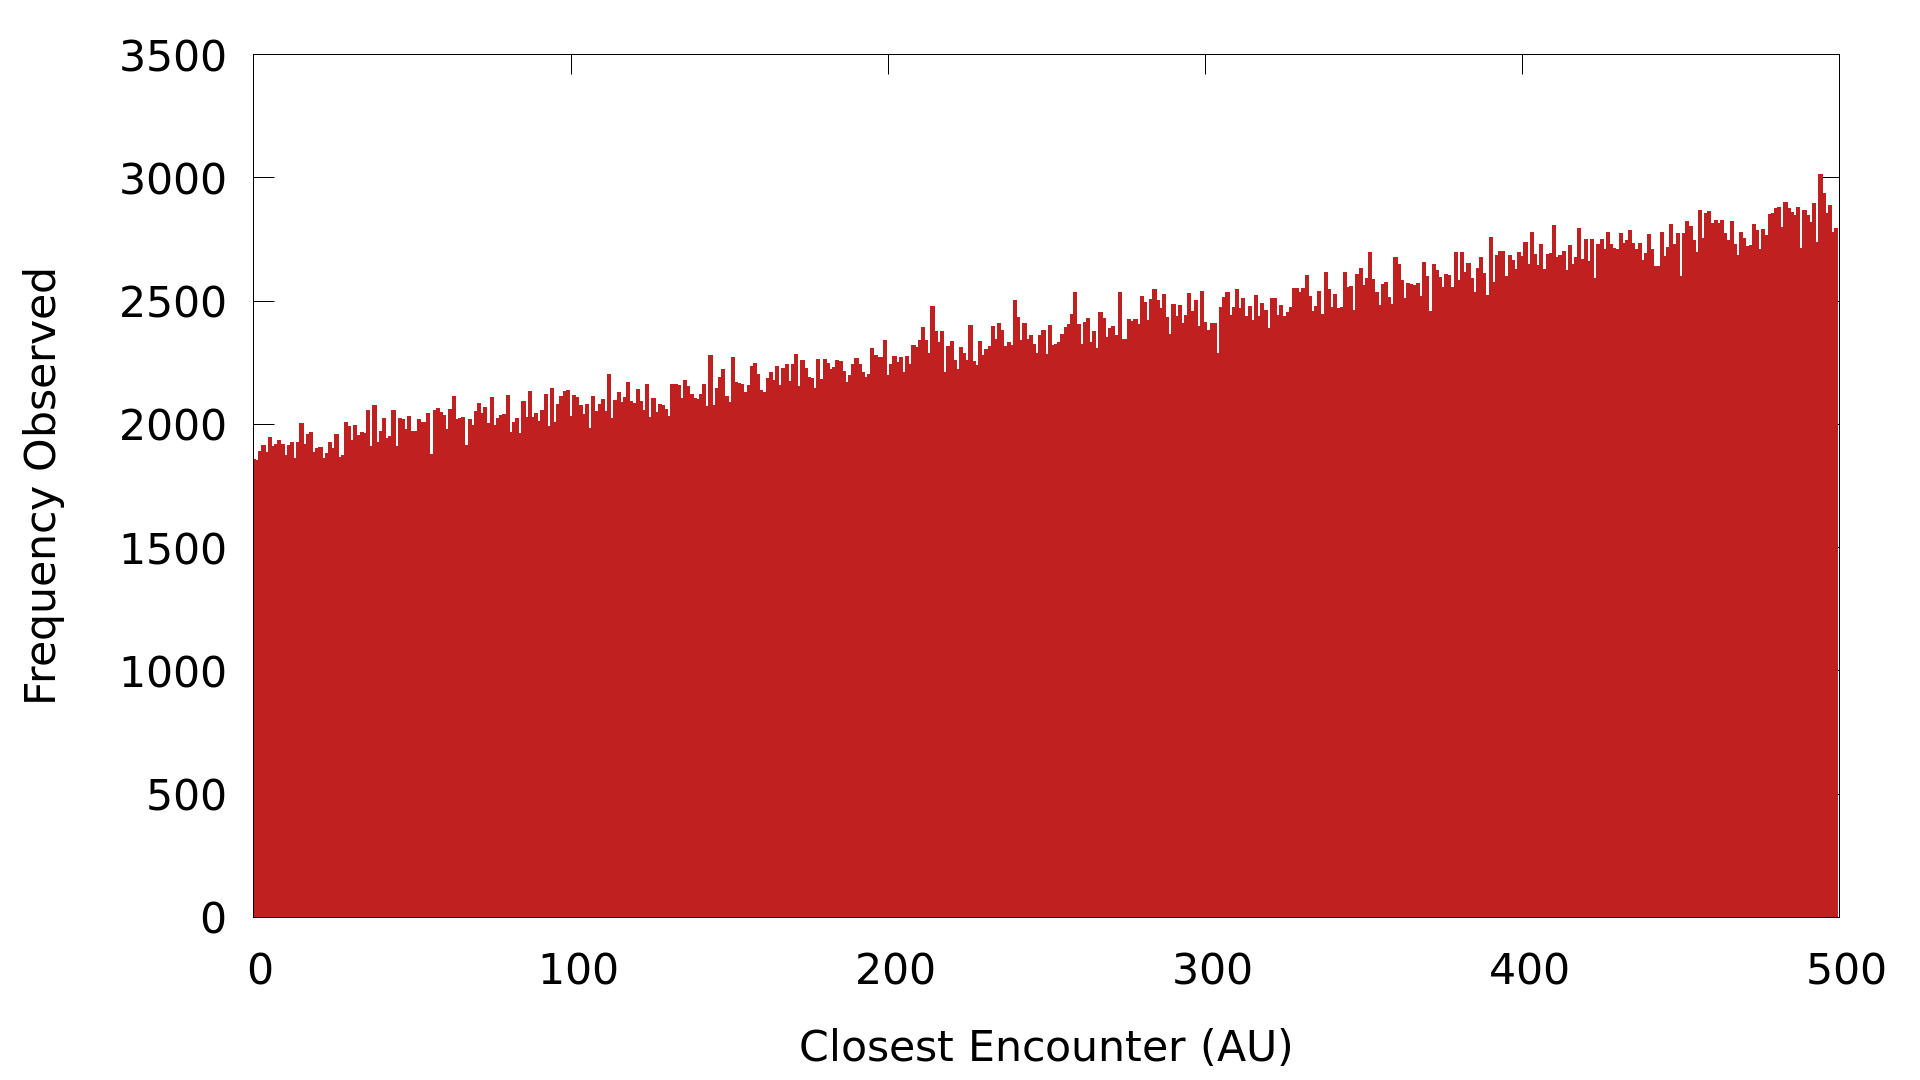
\includegraphics[width=3.25in]{encounter_distance_frequency_n1000} &
            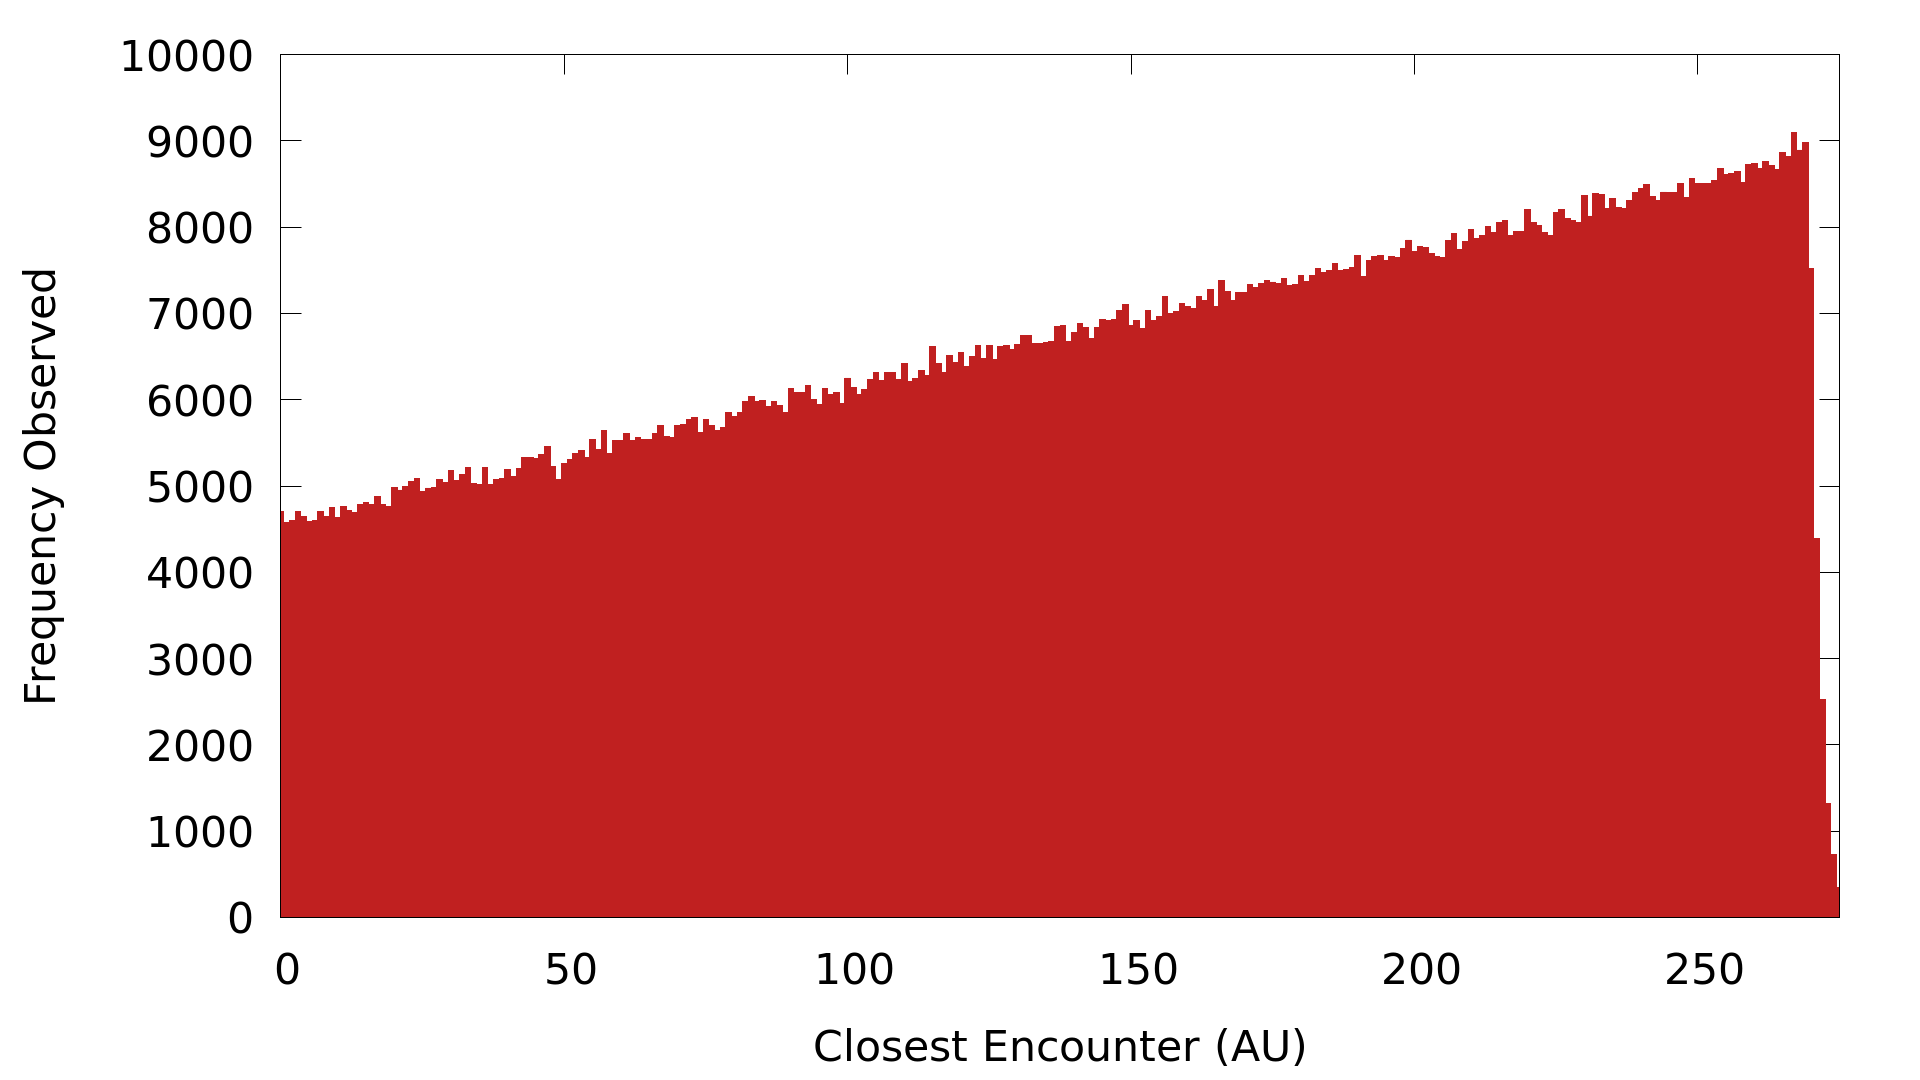
\includegraphics[width=3.25in]{encounter_distance_frequency_n4000}
        \end{tabular}
    \end{figure}

    \begin{table}[H]
        \centering
        \caption{Encounter statistics from the three sizes of clusters run.
            The total number of encounters observed as well as the number within
            two thresholds is listed.}
        \vspace{0.2in}

        \begin{tabular}{|cccc|}
            \hline
            \textbf{Cluster Size} & \textbf{\# Encounters} & \textbf{\# Below 100 AU} 
                & \textbf{\# Below 30 AU} \\
            \hline
            1000 & 1,831,075 & 198,952 (10.89 \%) & 57,351 (3.13 \%) \\
            2000 & 1,896,763 & 327,972 (17.29 \%) & 92,461 (4.87 \%) \\
            4000 & 1,869,983 & 534,999 (28.61 \%) & 144,231 (7.71 \%) \\
            \hline
        \end{tabular}
    \end{table}

    \subsubsection{Planetary System Simulation}

    The second stage of pipeline uses the cluster encounter data to do
    detailed analysis of individual encounters.
    From the cluster simulation, a list of star encounters for any number of 
    clusters may be generated. The next step is to read these encounters and
    simulate just the two stars involved for each in isolated from the 
    environment. In addition, planets are placed in orbit around both stars in the
    encounter before they are added to the simulation. The initial positions,
    velocities and physical parameters of the stars are identical to what they
    were at the moment AMUSE identified them as interacting. 

    Once the stars are setup with their planets, their gravitational dynamics
    are simulated. As the stars have just started interacting, the stars should
    move toward each other, reach a point of closest approach and then separate again
    in hyperbolic orbits. When the two stars separate to a distance farther than
    apart than they started, the simulation is stopped and the final states of the two
    systems are recorded. 

    As previously stated, each hundred megayears of a cluster simulation yields over
    one hundred encounters, but most of these encounters are completely uninteresting
    in their planetary dynamics. So for these simulations, the list of encounters is 
    first filtered so "uninteresting" interactions are removed. For an Earth-Jupiter
    system, a closest approach of 30 AU was chosen as the farthest periastron to be
    worth considering. With this cut in place, only ten to twenty encounters, on
    average, are left per 100 megayears of cluster simulation.

    %TODO: If more distant planets added, 30 AU limit must increase.

    Each individual two-system simulation requires only twenty to thirty
    seconds of clock time to run on the computational cluster. This can be
    parallelized easily and we were able to run as many as fifty
    planetary simulations at once. With the 30 AU cut, all relevant encounters 
    in a single cluster simulation can be simulated within ten minutes.

    The planets added to the stars were kept consistent throughout, thus 
    each star in each simulation was made to have one Earth and one Jupiter
    orbiting with the approximate physical and orbital
    parameters as the respective planets in our solar system. 
    In this way, all variation will occur through variations in the clusters, not
    the planetary systems.
    All planets are
    placed in circular orbits (with $e=0$), making it easy to analyze
    any changes after the interaction.
    %TODO: Orbital planes

    When the simulation is finished, the data important for later analysis is
    saved. The most important of this data is the starting and ending
    orbital elements, as well as the initial and final positions of each of the bodies.
    Additionally, the trajectory of all bodies may be saved in detail. 
    The trajectories are useful for replaying an individual encounter or plotting the
    interaction to manually analyze some of the particularly interesting 
    encounters.

    We analyzed 55,000 close encounters for each cluster size. 
    Figure \ref{fig:planet_simulations} illustrates two examples of close encounter
    events. These two examples are chosen from the thousands of simulations
    that were run in the database. The large hyperbolic trajectories are the 
    two stars interacting while the helices around them are the planets. In these
    interactions, the stars approach extremely close, within 2 AU in both cases, and
    the planets are significantly affected. These two samples represent only
    a snapshot of the full set of interactions that occur within the simulations.

    \begin{figure}[H]
        \centering
        \caption{Two examples of close encounter events. On the top, we see
            an ejection of two planets from the systems. On the bottom, one planet
            in the first system is captured by the second and approaches 
            within 0.5 AU of the star. In both cases, the
            orbits of the remaining planets become more eccentric.
        }
        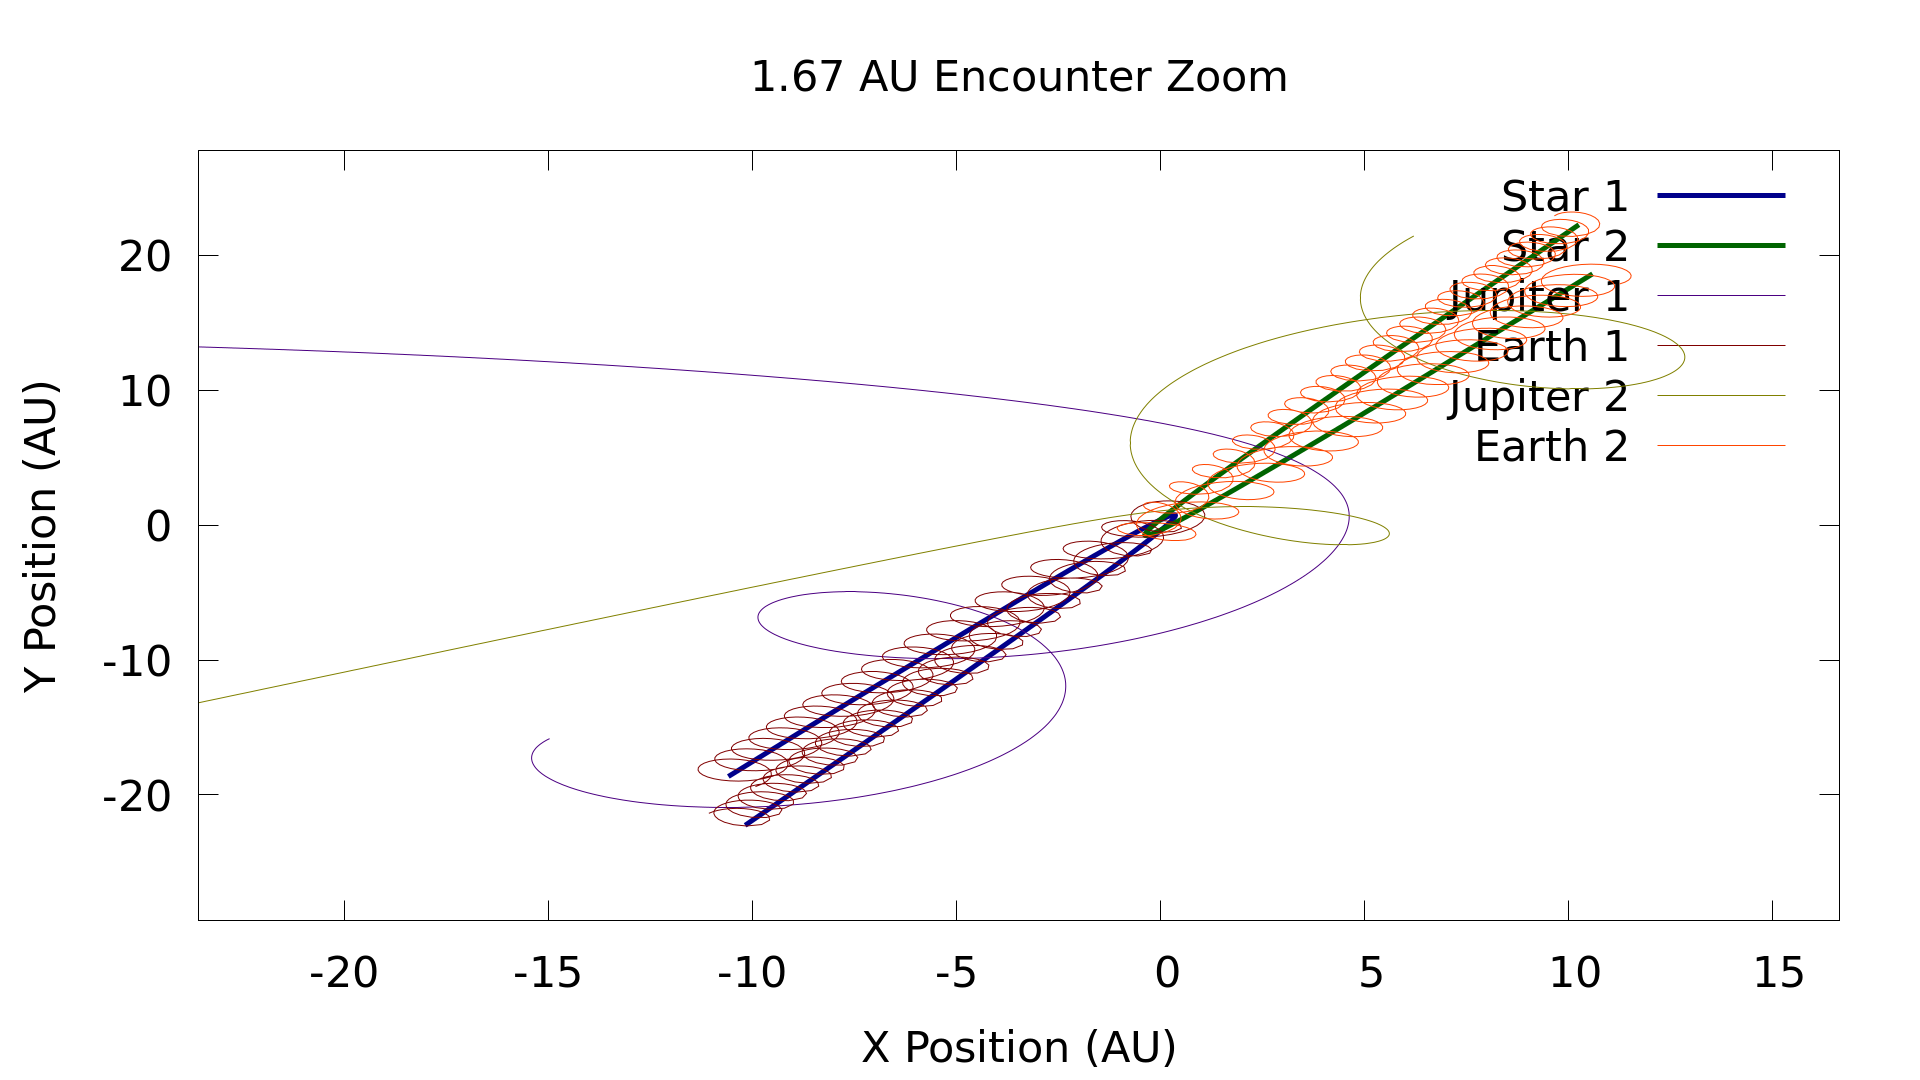
\includegraphics[width=5in]{1_67_AU_zoom}
        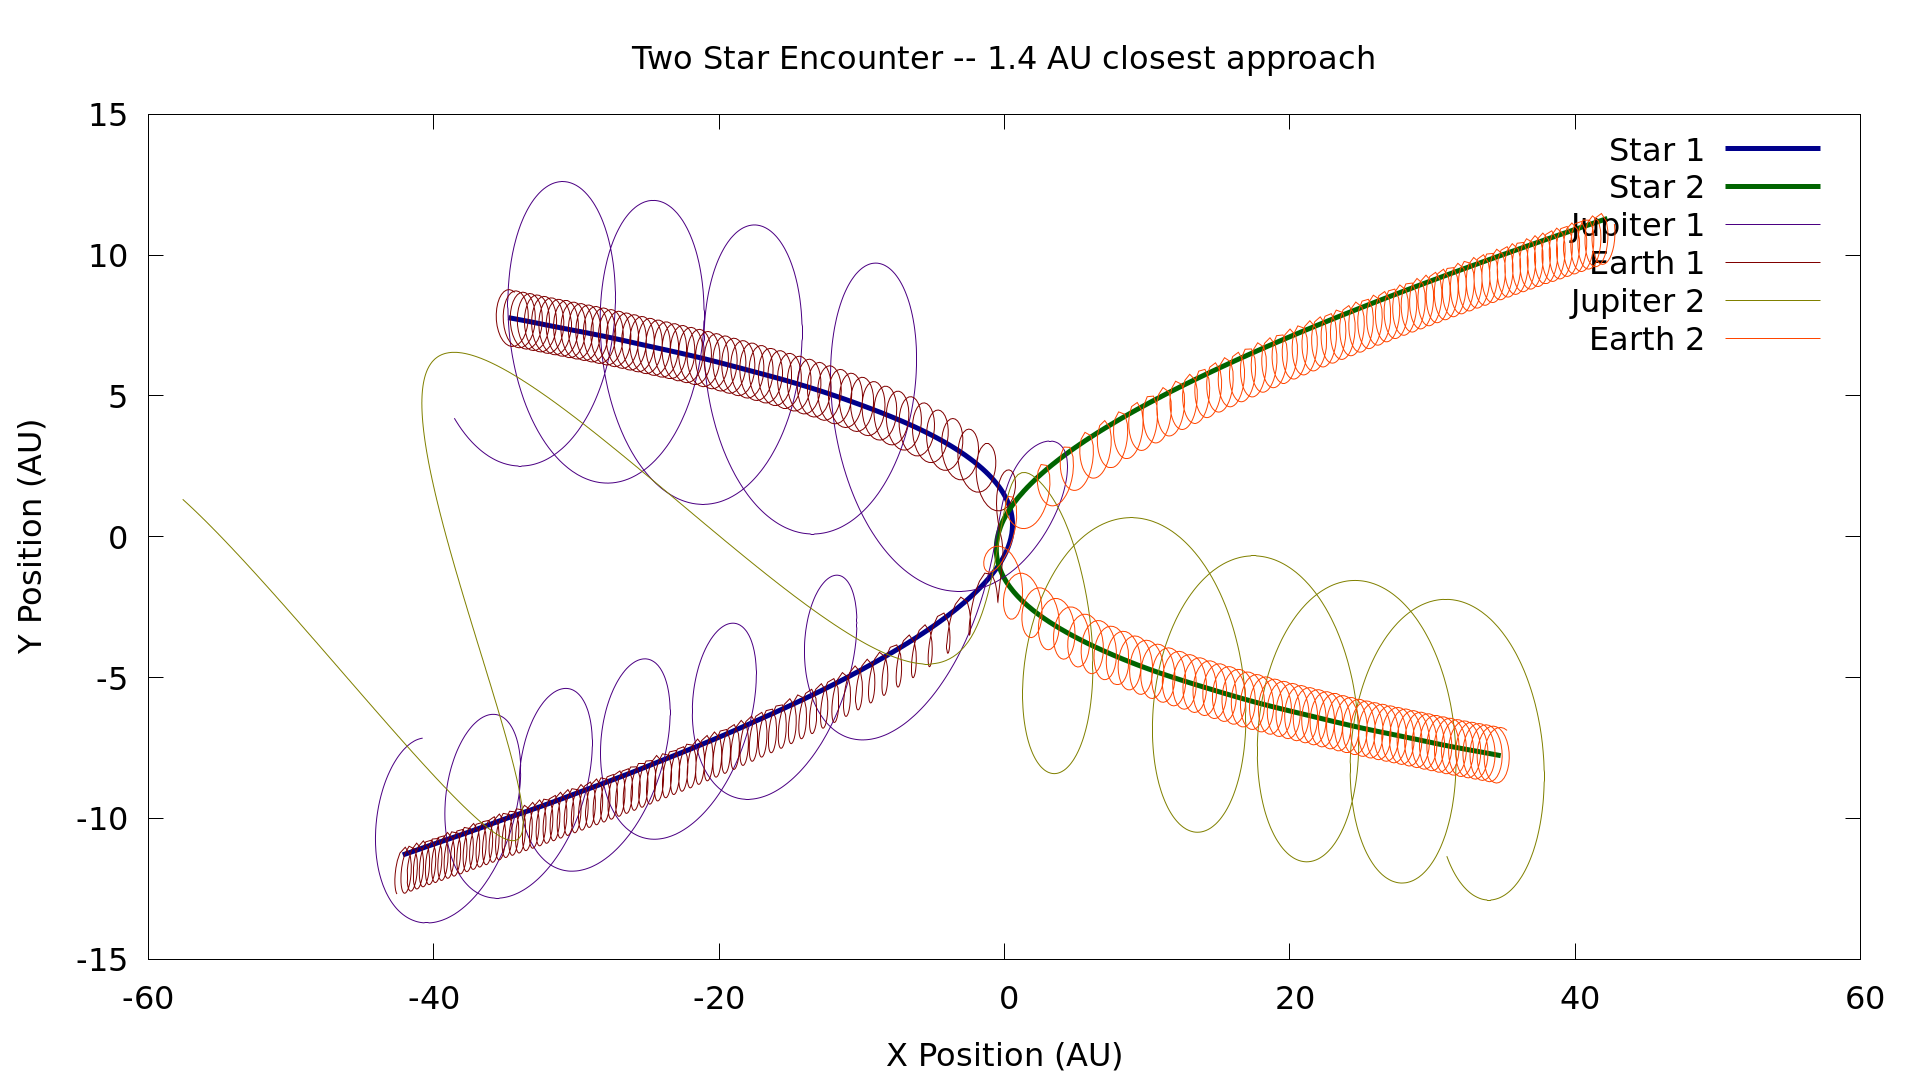
\includegraphics[width=5in]{1.4AU/1_4_AU_encounter_plot}
    \end{figure}

    \subsubsection{Data Analysis}

    The final stage of the pipeline is to actually analyze the encounter data 
    output by the previous simulations. After a few days of running simulations,
    we are able to obtain nearly one-thousand %TODO: Number, update
    close encounters simulated
    for analysis. The database constructed for this process allows all of the
    encounters to be loaded and related back to their originating clusters.

    There are numerous potentially interesting trends or situations to look for in
    the output, some of which are beyond the scope we explored. 
    
    One very simple analysis we perform is to look at the output
    eccentricities. Since all planets were given $e=0$ initial orbits, any deviation
    from zero in the output is an effect of the interaction. This shows not only the
    approximate amount an orbit was disturbed, it also shows planets that were ejected
    from their original system. Additionally, by computing the eccentricity between
    each planet and \textit{both} stars, we are able to determine how many planets are captured
    by the approaching star.

    A second analysis is to look at the final periastron for all planets that are still
    gravitationally bound (that is, final $e<1$). Jupiters with a periastron
    of only a fraction of an AU are prime candidates to become Hot Jupiters. Additionally
    any significant periastron change in the Earth may have significant consequences
    to the sustainability of life.

\section{Data Pipeline and Storage}

    \subsection{Database}

    One pervasive problem in running a large number of simulations for analysis is
    that there is a large amount of data created and all of this data needs to be
    organized in order to perform detailed analysis. For instance, different simulations
    needs to be kept separate and the parameters used to create the clusters initially
    needs to be known. Additionally, if changes are made to any part of the process, it
    is necessary to keep that data apart from the previous data.

    A second important consideration for this project is that the simulations themselves
    can be run in parallel and in large numbers. Big runs take a long time to run
    and thus it would be highly beneficial to be able to simultaneously run cluster
    simulations, run planetary system encounter simulations and analyze all of the
    completed simulations without worrying about the processes interfering with one
    another or using only partially complete data.

    In order to address all of these concerns, we developed a python library 
    for writing, maintaining and reading a database of this information. This database
    creates one directory for each cluster that is simulated. Within each directory,
    there is a table of all encounters, a table of the initial states of all stars
    and a set of details about the run itself. These directories are separated
    into clusters of the same initial cluster parameters for easy segregation if needed.

    When simulations of the individual encounters are performed, each encounter
    creates a subdirectory inside of the originating cluster's directory for the 
    results. 
    The initial and final parameters of each body in the simulation are stored, along
    with trajectories for the particles during the encounter. When all simulations
    in some cluster are complete, overall statistics about which encounters were
    simulated and which were skipped due to data cuts are generated.

    In each of these processes, the program first creates a "lock" file before it
    writes any data to the database. This lock file signifies that the cluster or
    encounters within are being actively simulated by some program at the time and
    should not be touched by anything else until it is removed. This allows us to
    safely achieve the high level of parallelisation desired without risk of data
    corruption. The lock file stores the time it is created so if a program
    crashes, power is lost or some other event that causes the program to end without
    proper termination, a lock can be identified as old automatically which 
    signals that the data contained within is likely incomplete and the program
    writing it was unable to properly complete.

    One final data management feature is the inclusion of a database version number
    in each summary file produced. This allows for the data format to be modified,
    additional features to be added and backward incompatible changes to be introduced
    without making all old data unusable. 

    It is our hope is not only that this makes our data analysis tasks easier, but
    that it is usable by future researchers who want to perform similar experiments.

    \subsection{Analysis}

    As hundreds of thousands of encounter simulation results can be stored
    in the database, and a few kilobytes of data is stored for each, 
    it can take as long as a half-hour to load, parse process each set of 100,000 results.
    In order to promote modularity, each analysis should be able to run independently
    of all others, but running each analysis independently over all the data would result
    in as much as an order of magnitude slow down as the data would be parsed again and
    again. However, on the opposite side, throwing all analyses into a single function or
    module makes it very difficult for future scientists to define their own analyses
    without understanding everything already done or replacing it all entirely. 
    Additionally, it becomes extremely difficult for multiple people to collaboratively
    write analyses.

    To remedy the problem without losing modularity, the analysis module takes a
    set of analysis tasks to run. Each analysis task has a coroutine that accepts a
    single encounter result at a time, and incrementally processes that data into 
    its isolated state. This technique (called an "online algorithm") allows any number
    of analyses to be performed in one pass over the input data. The complexity of writing
    an analysis using this approach is slightly higher, and requires code be written
    to understand this model, but the end result is a fast and modular processing framework.

\section{Results}

    To draw conclusions and generate plots, we used exactly 55,000 close encounters from
    each set of parameters.

    We first analyze the final planet eccentricities. Figure \ref{fig:eccentricies} shows
    the resulting spectrum of eccentricity values after the simulation. The eccentricity
    values are divided into 100 bins, each 0.01 wide. The top pair
    of plots is for 1000-star clusters, followed by 2000-star and 4000-star clusters.
    The green plots show Earths while the blue plots show Jupiters. The Jupiters are
    clearly more easily perturbed than the Earths, however a measurable number of Earths,
    at least a few hundred, are perturbed to have an eccentricity greater than 0.5. In both
    cases, the vast majority of planets are hardly perturbed at all, with tens of thousands
    of final states having $e<0.1$.

    \begin{figure}[H]
        \centering
        \caption{Final orbit eccentricity frequencies for the planets 
            after the two systems interact. The left plots are for the Earth and the right
            are for the Jupiter. The frequency scale is base-10 logarithmic.
            Planets that were ejected from their systems are not included.
        }
        \label{fig:eccentricies}

        \begin{tabular}{cc}
            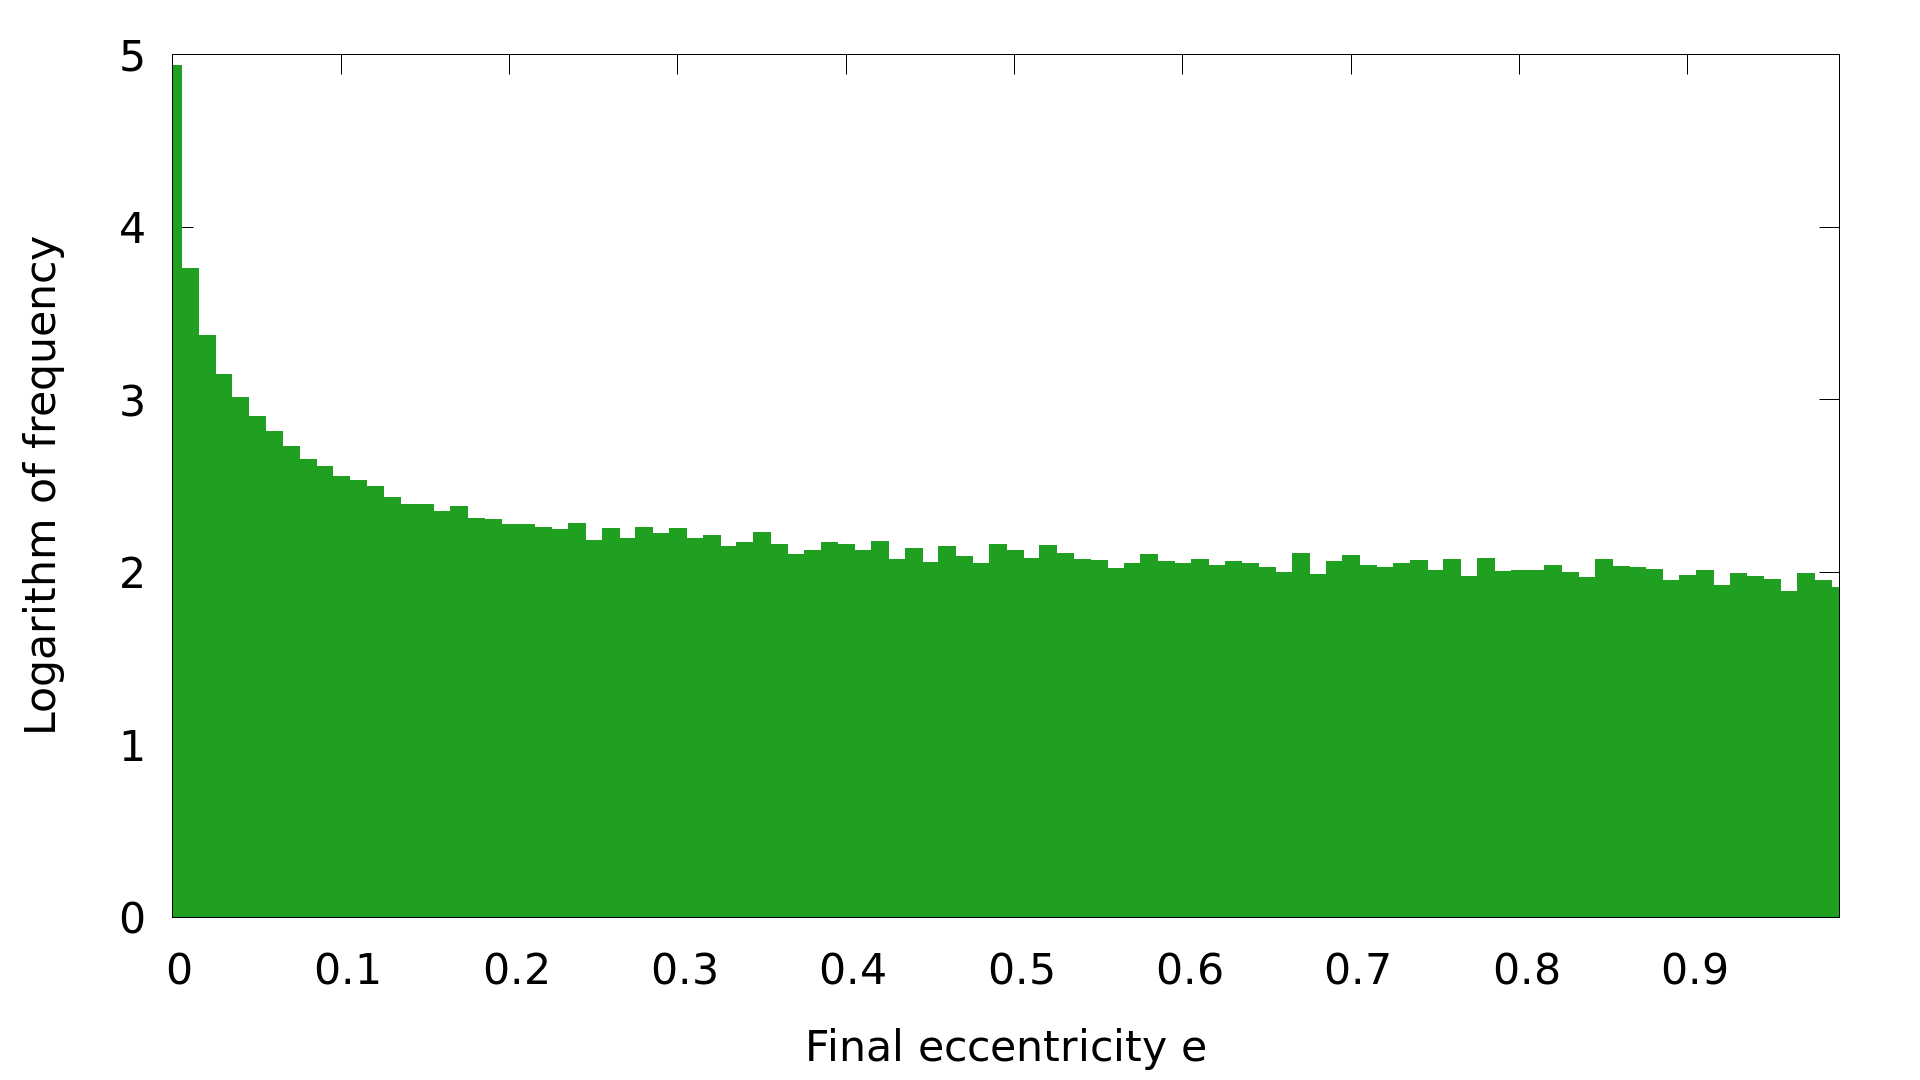
\includegraphics[width=3.25in]{eccentricity_earth_1000} &
            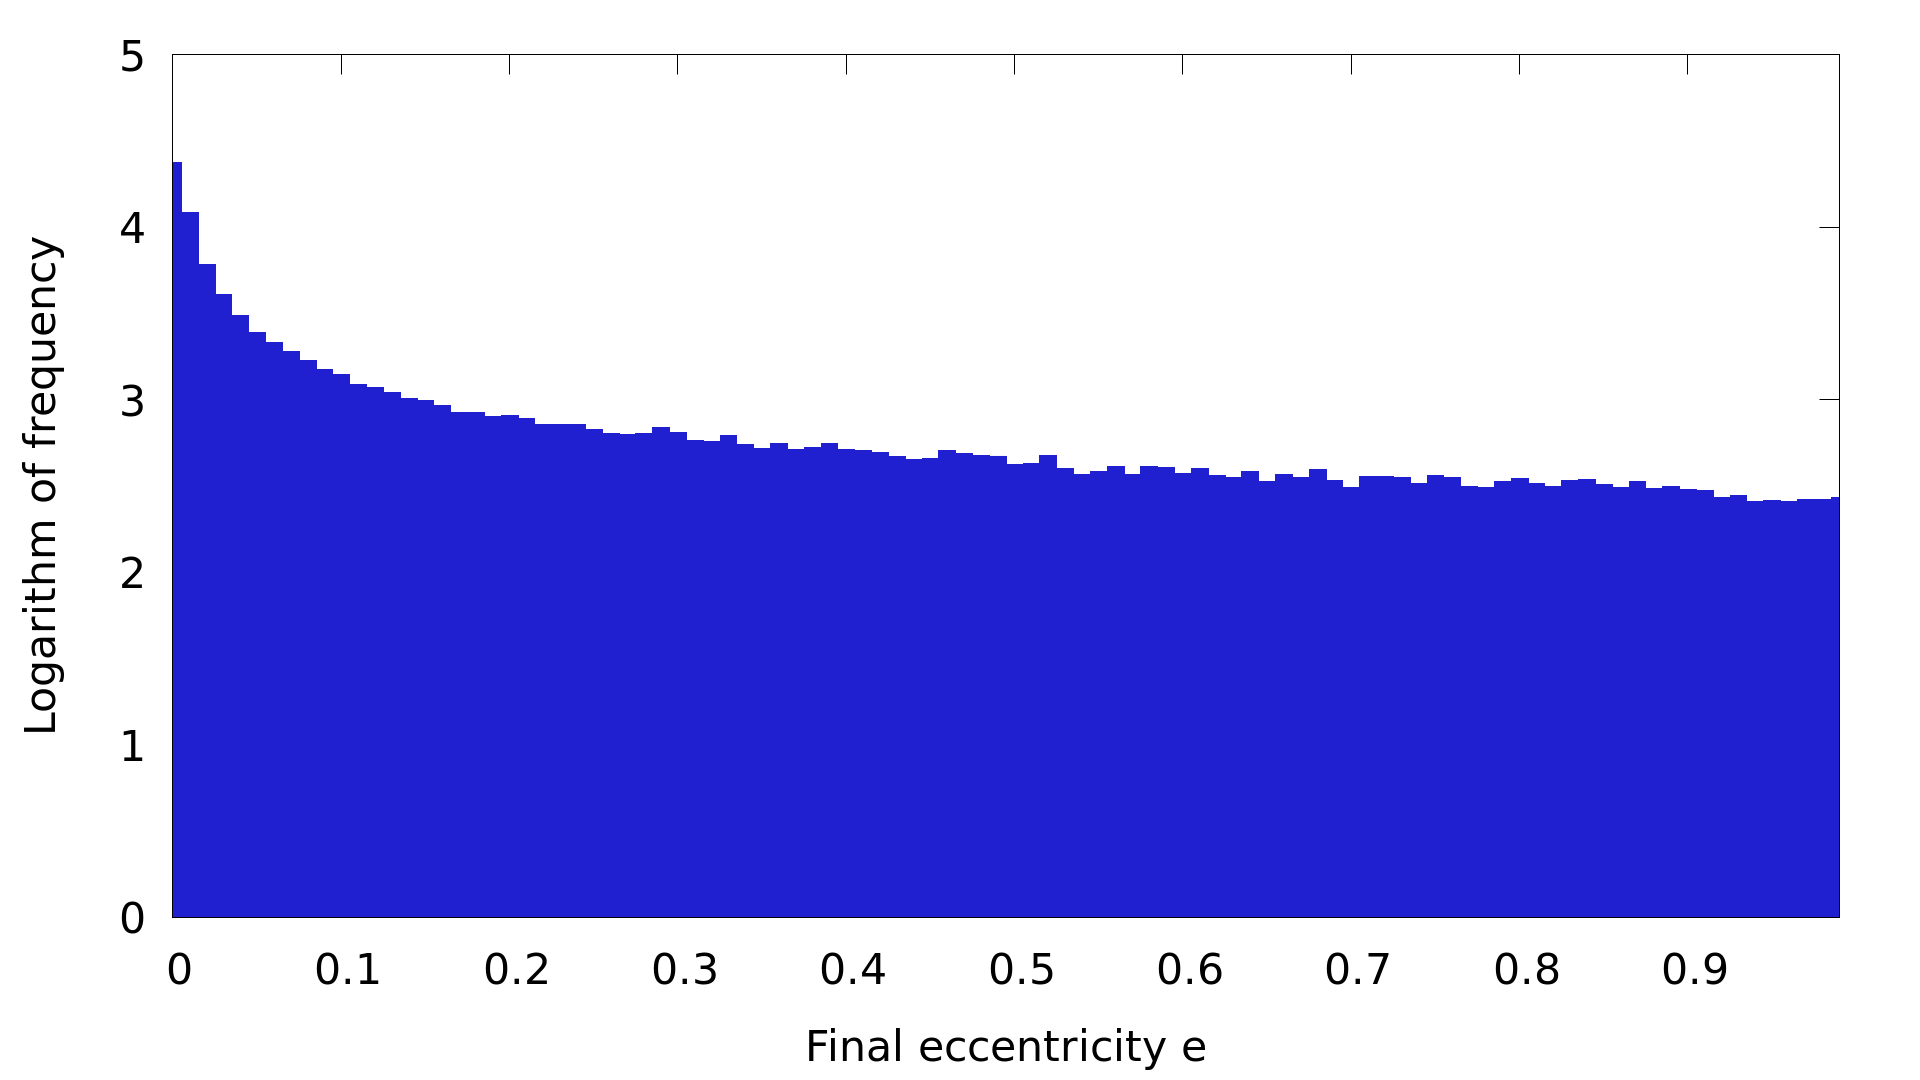
\includegraphics[width=3.25in]{eccentricity_jupiter_1000} \\

            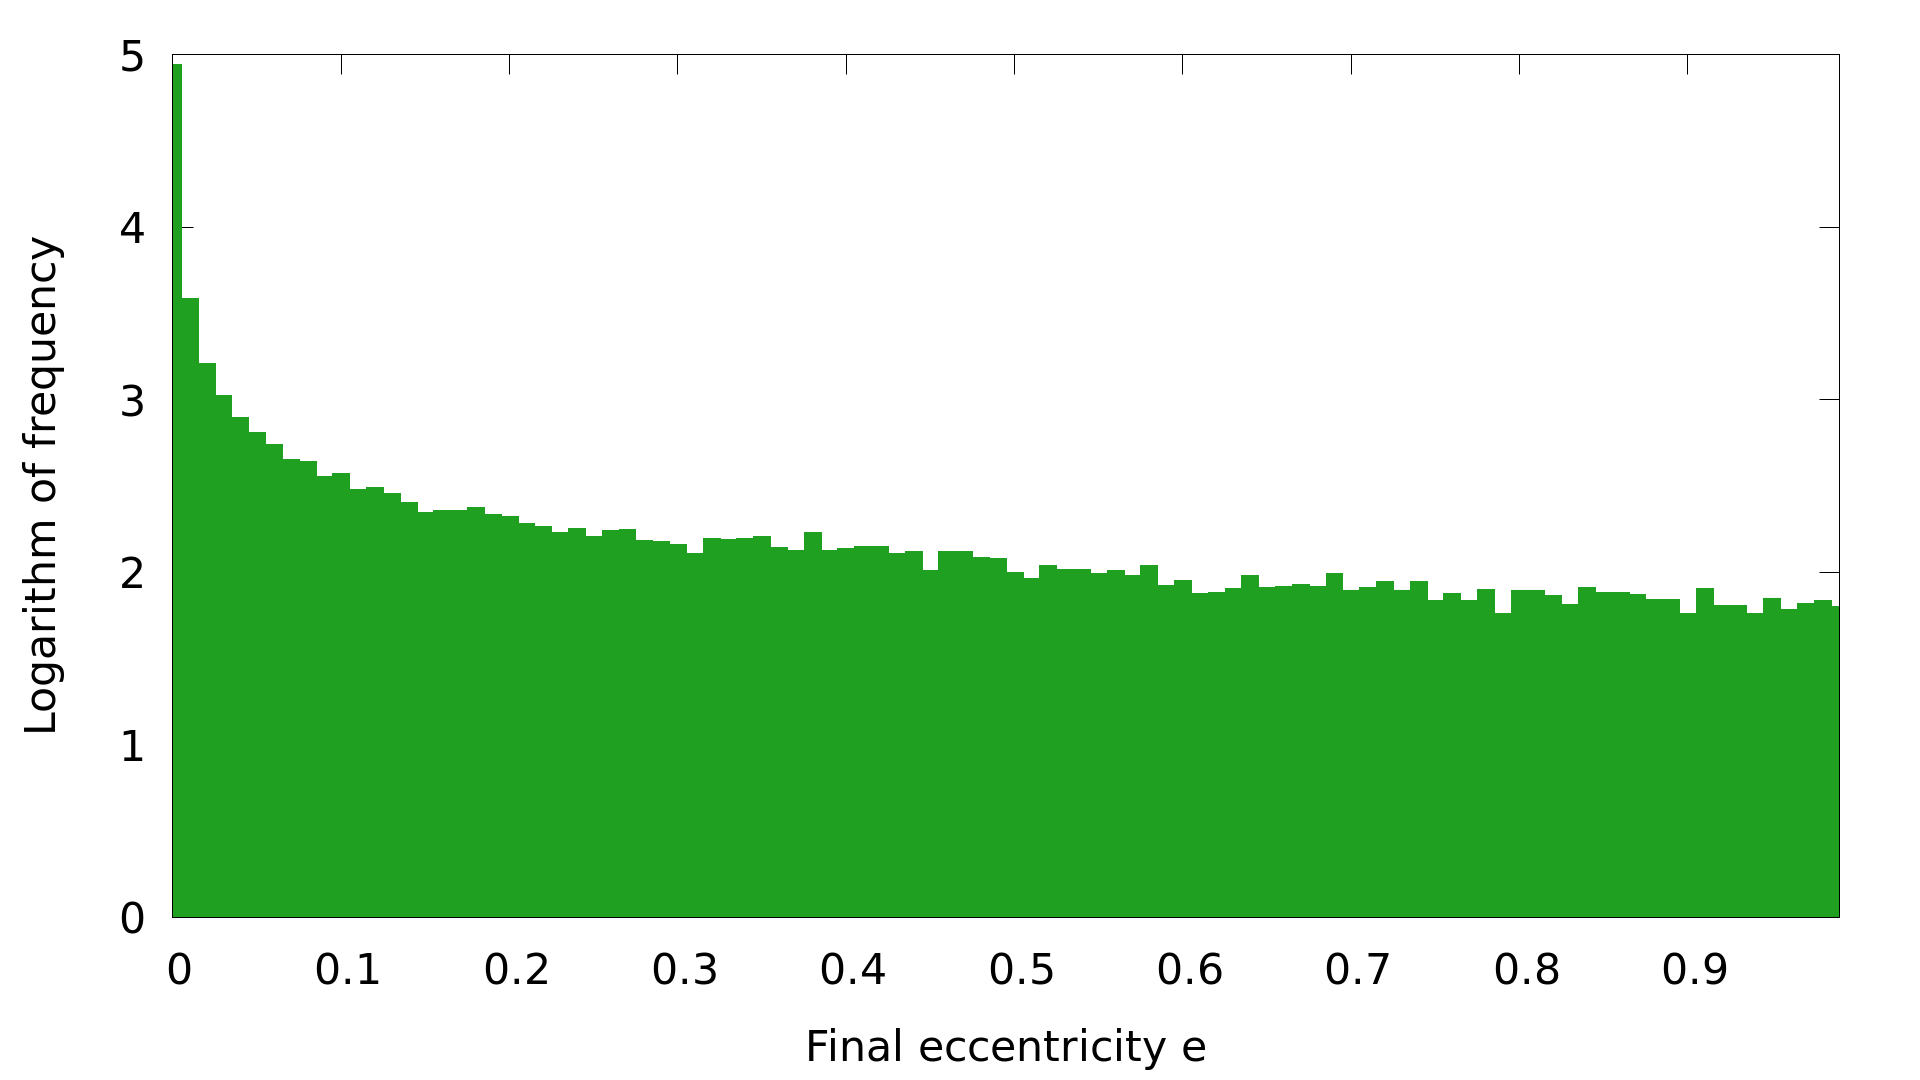
\includegraphics[width=3.25in]{eccentricity_earth_2000} &
            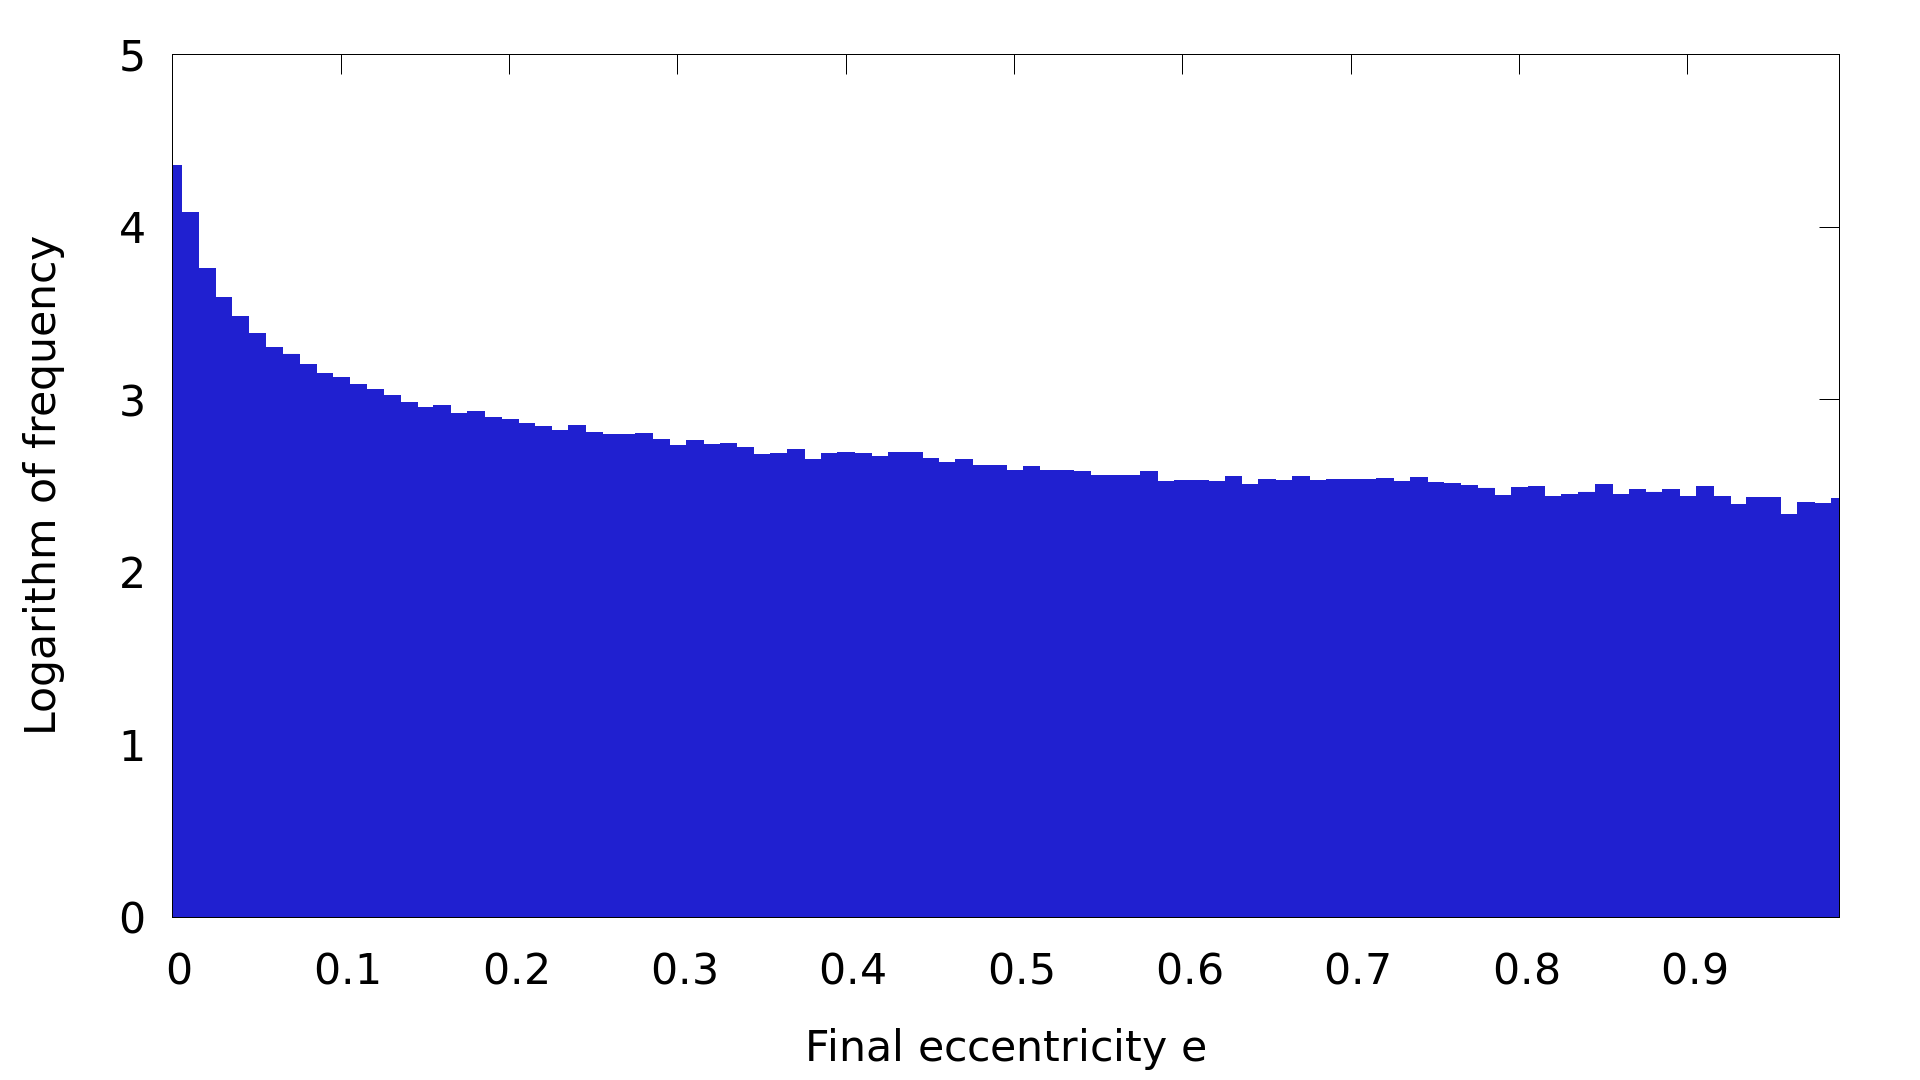
\includegraphics[width=3.25in]{eccentricity_jupiter_2000} \\

            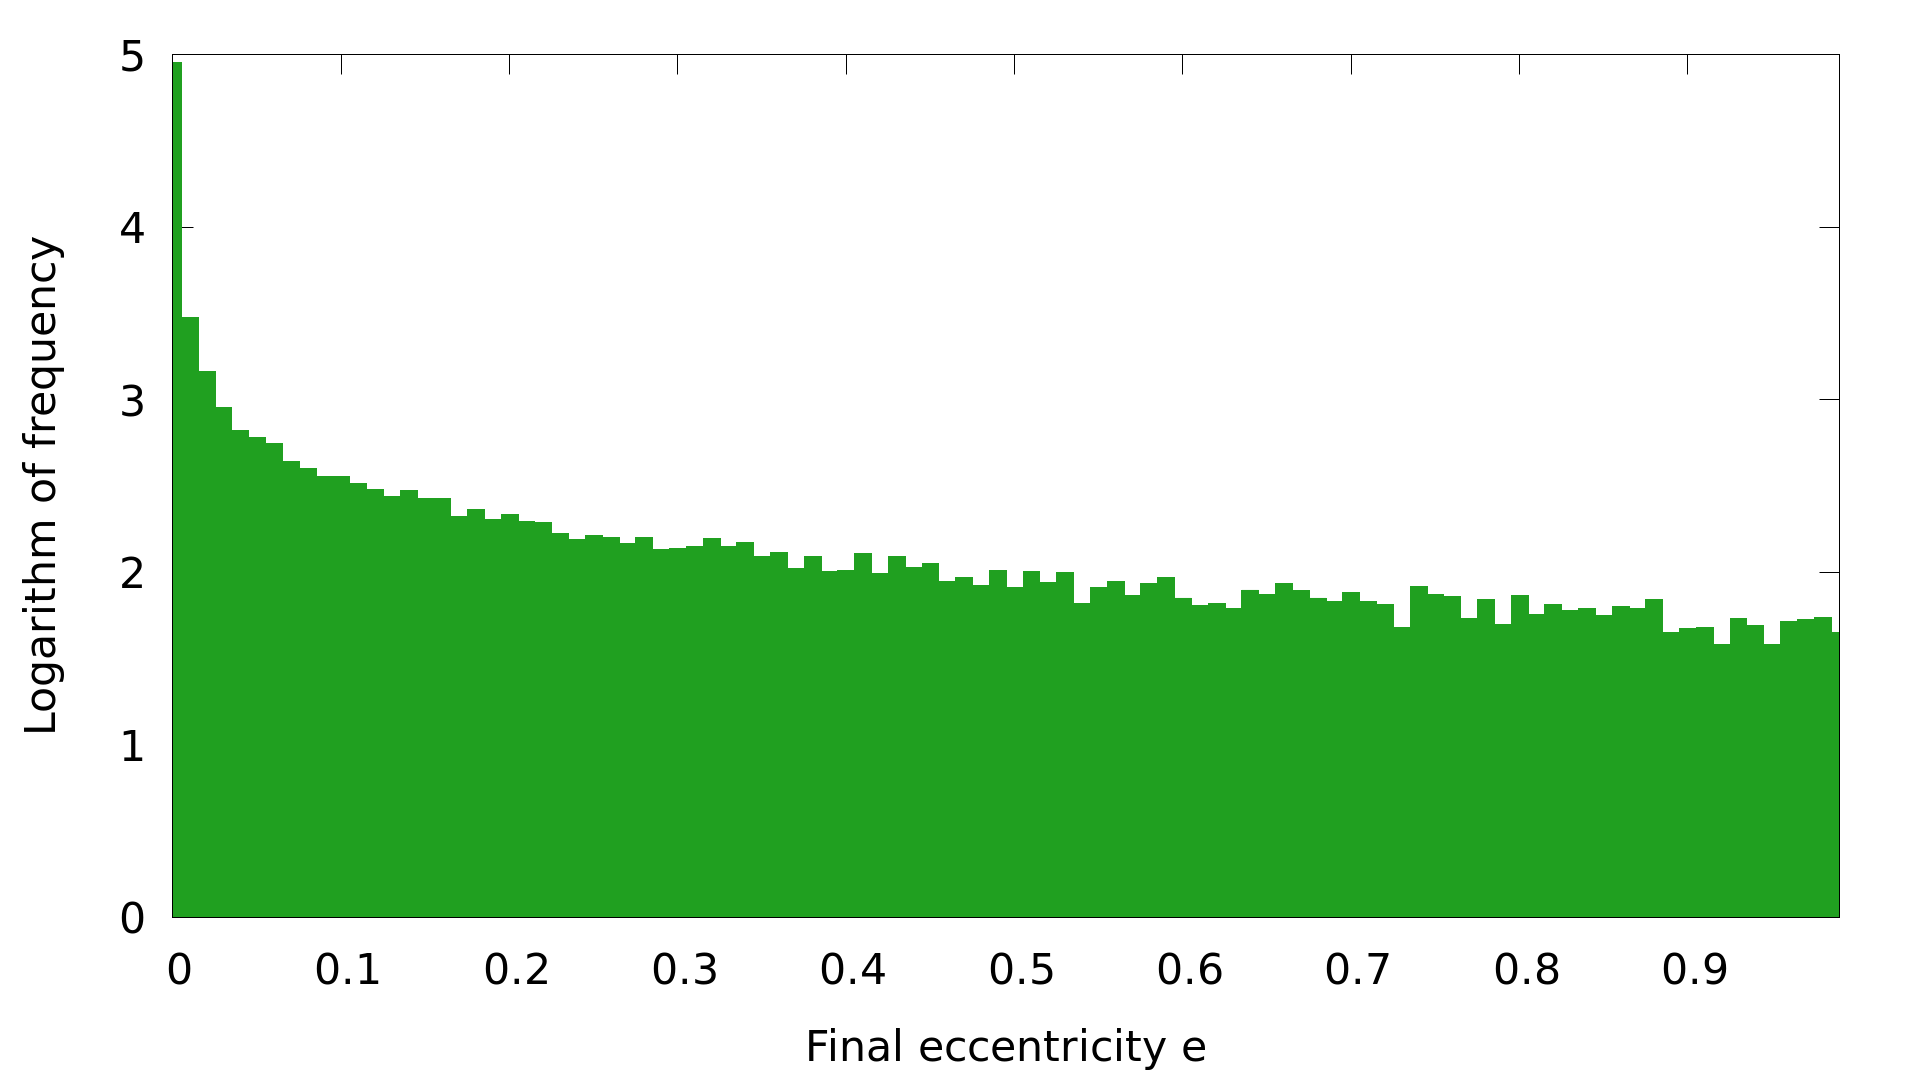
\includegraphics[width=3.25in]{eccentricity_earth_4000} &
            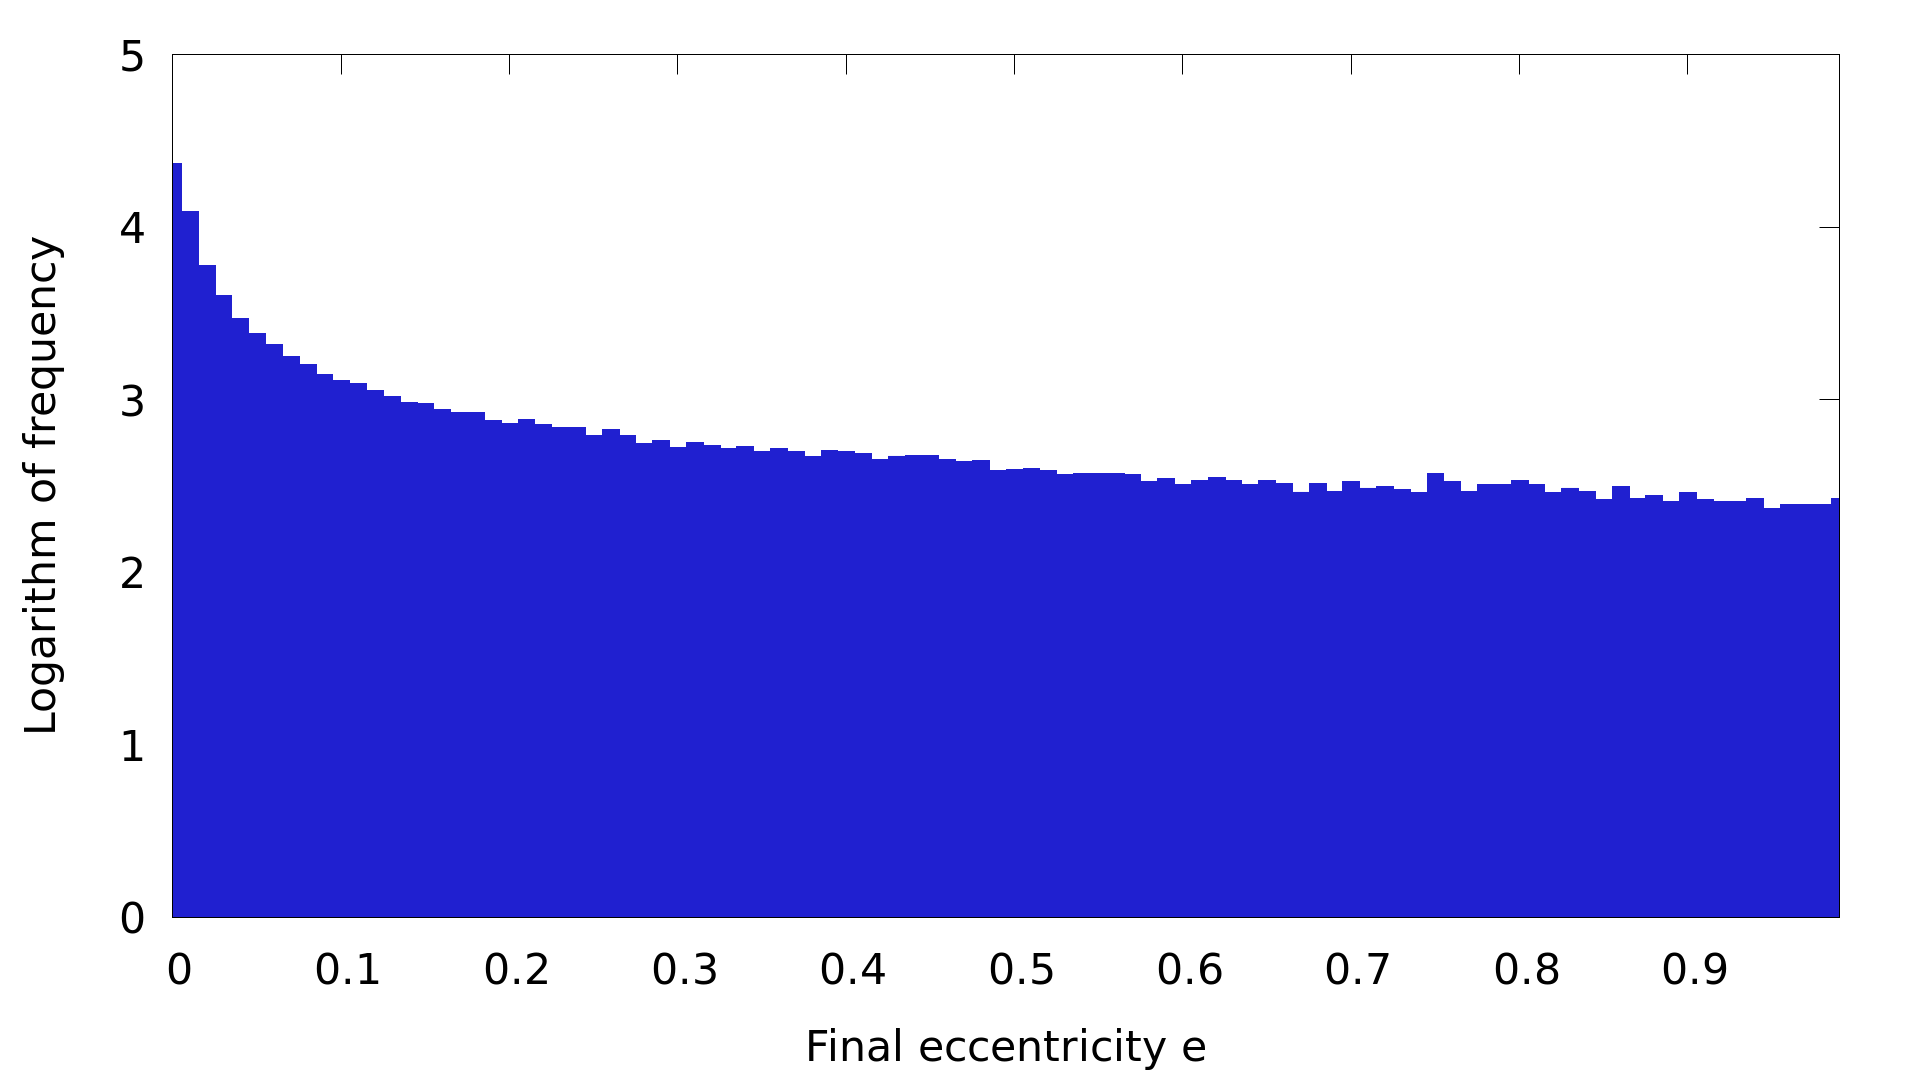
\includegraphics[width=3.25in]{eccentricity_jupiter_4000}
        \end{tabular}
    \end{figure}

    Figure \ref{fig:periastron} shows the final distributions of closest approaches.
    The top plots are 1000-star clusters, while the bottom are 4000-star clusters.
    There is a decrease in very close periastron distance with increasing cluster size,
    especially in the Earths. We find several hundred Jupiters with a periastron less than
    0.1 AU. The bottom-most plot is a zoom of the closest Jupiters for a 1000-star cluster.

    \begin{figure}[H]
        \centering
        \caption{Closest approaches of all Earth and Jupiter planets after 
            the encounter that have not escaped. On all plots, there is a peak
            at the unperturbed orbital distance (5.1 AU for Jupiter, 1.0 AU for
            Earth) and then a tail of closer approaches representing
            orbits that were more severely perturbed. Jupiter planets below 1.0 AU
            come into the inner planet orbits and could continue to interact further.
            The extremely close orbits potentially could become Hot Jupiters after
            orbit decay.
        }
        \label{fig:periastron}
        \begin{tabular}{cc}
            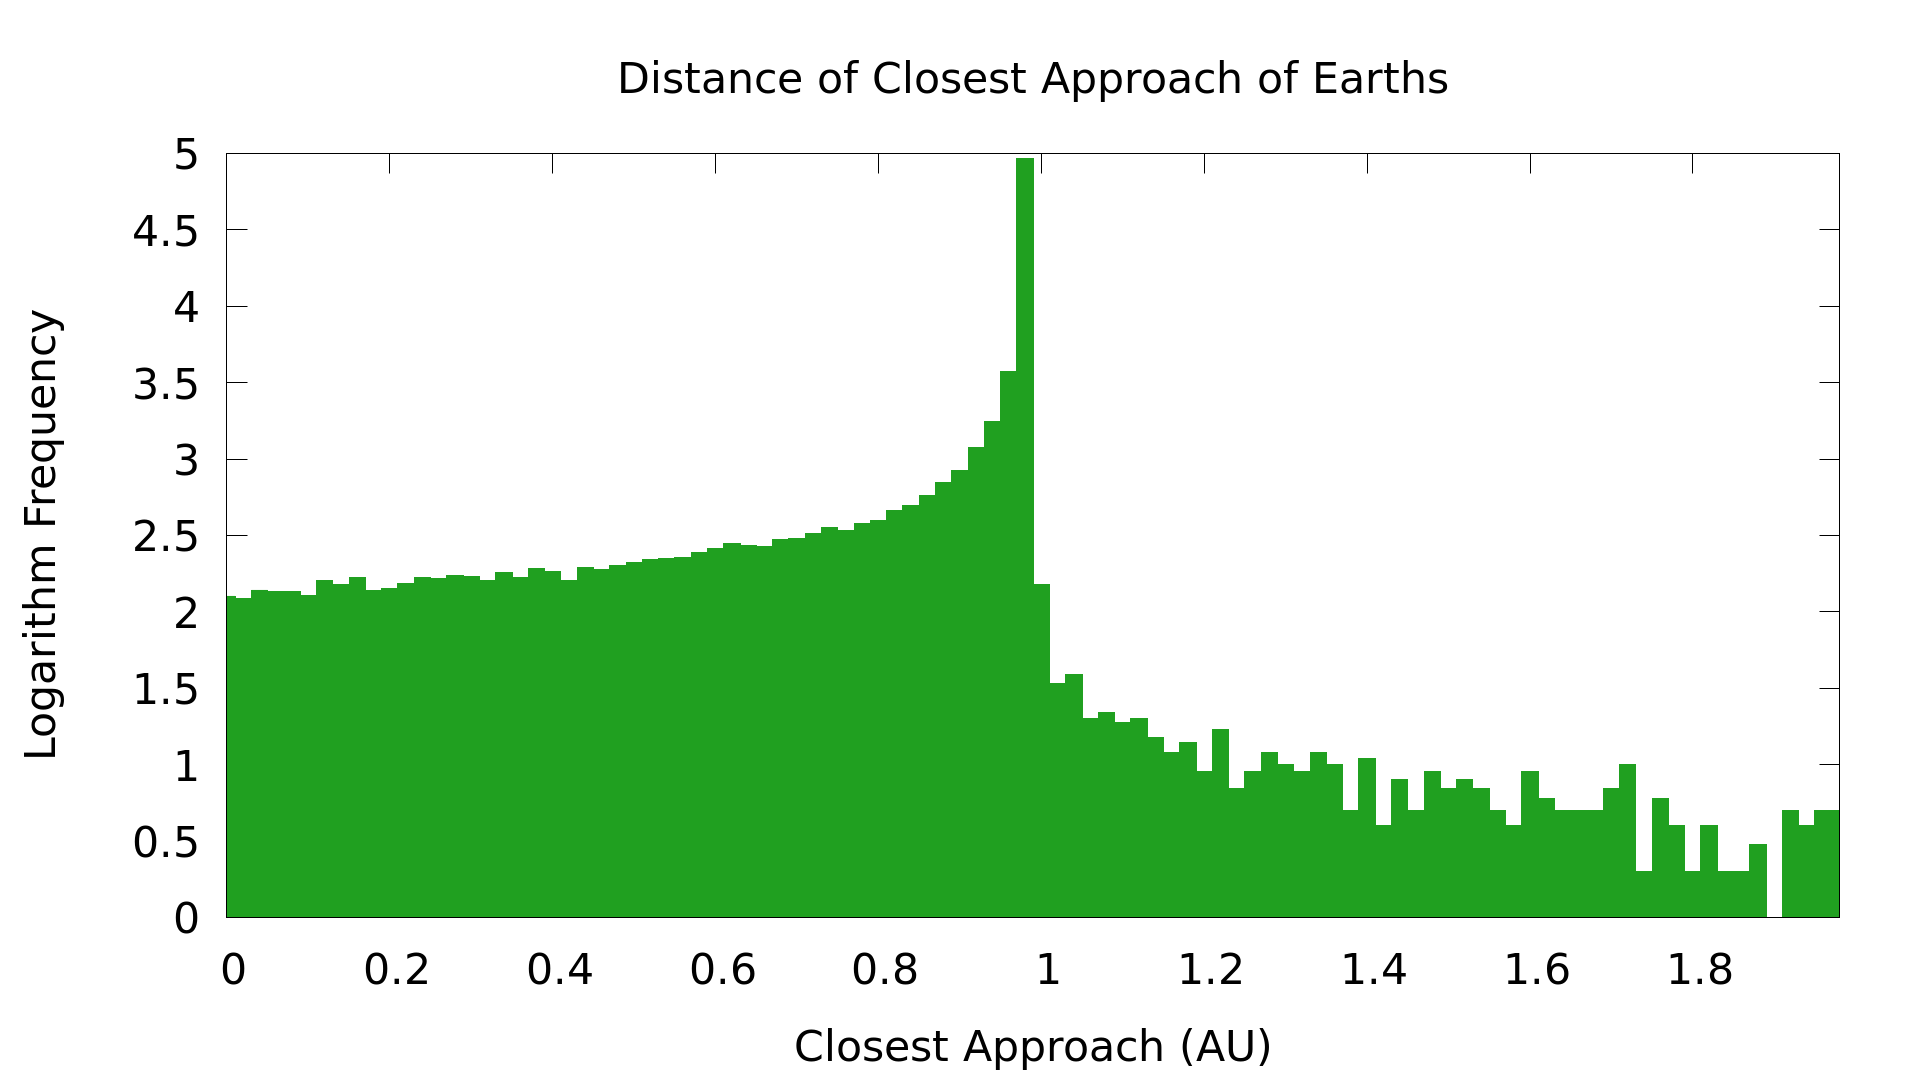
\includegraphics[width=3.25in]{periastron_earth_1000} &
            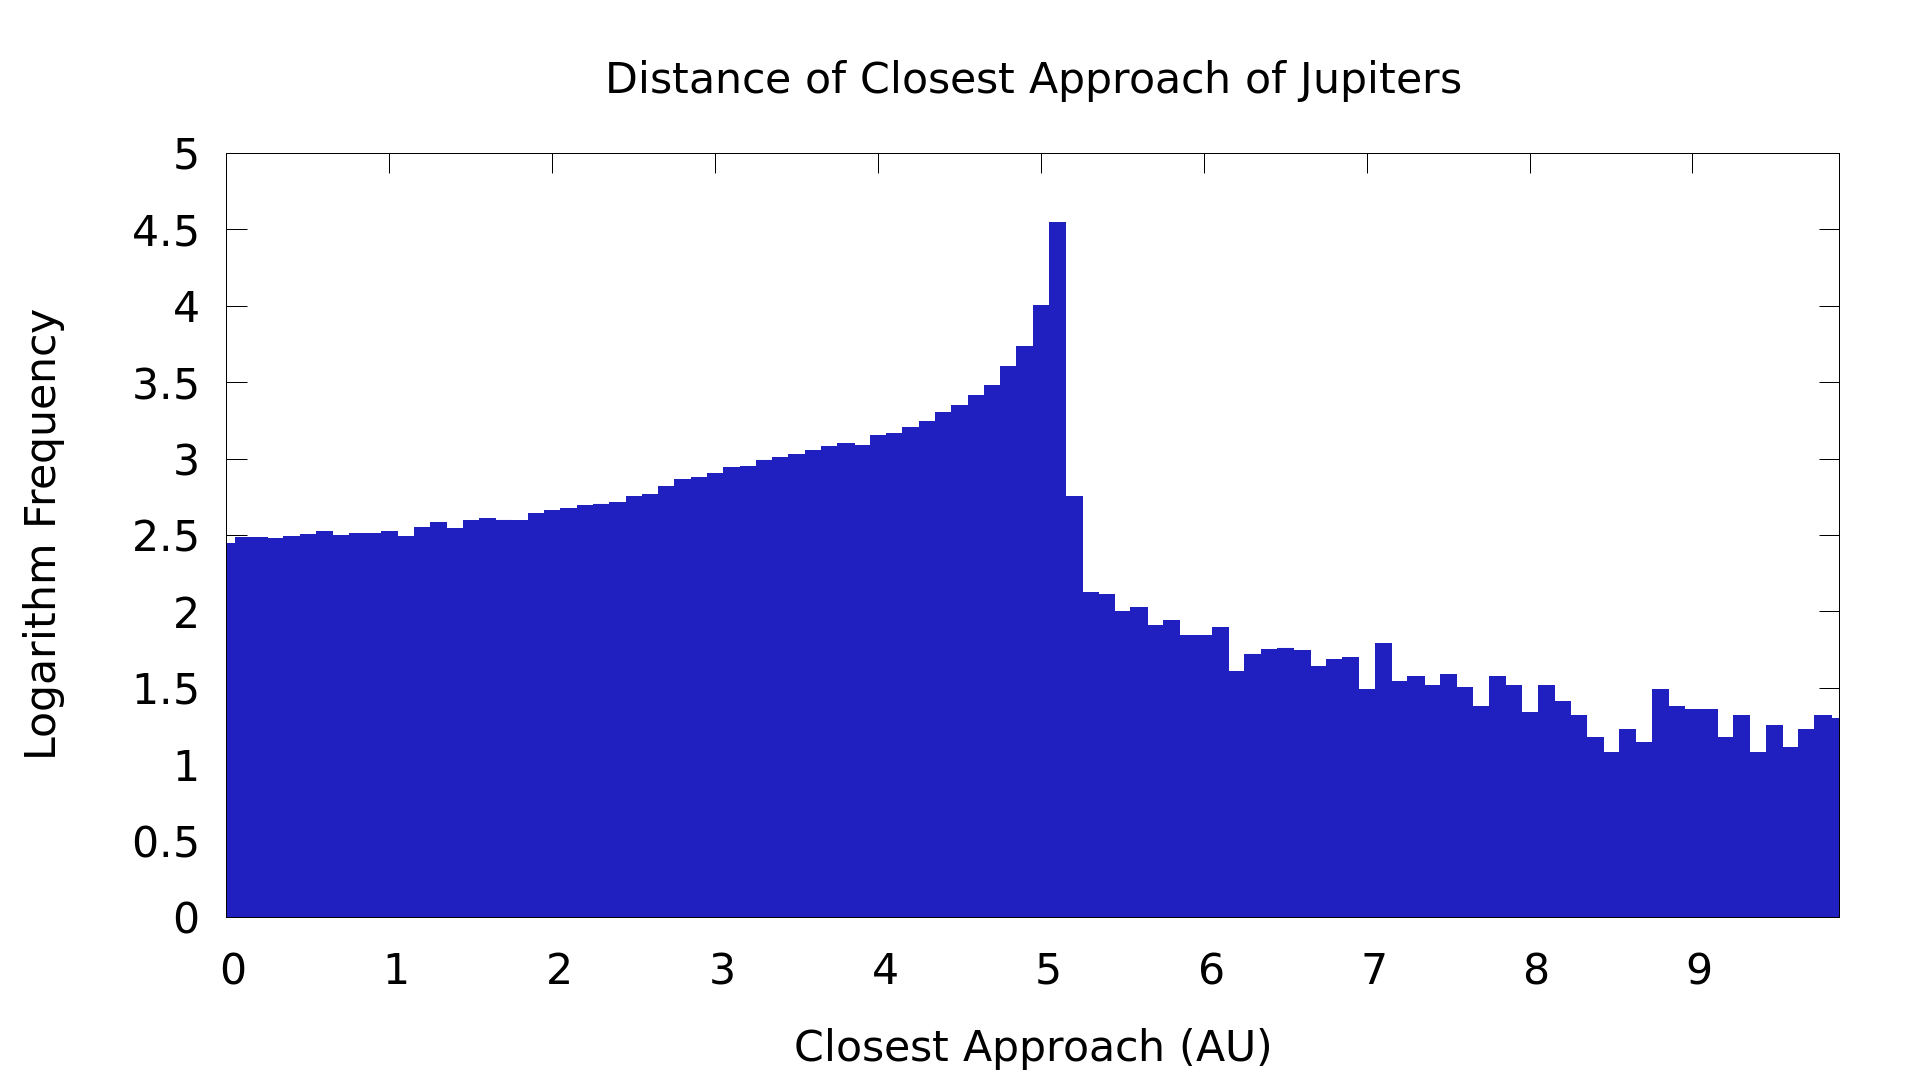
\includegraphics[width=3.25in]{periastron_jupiter_1000} \\

            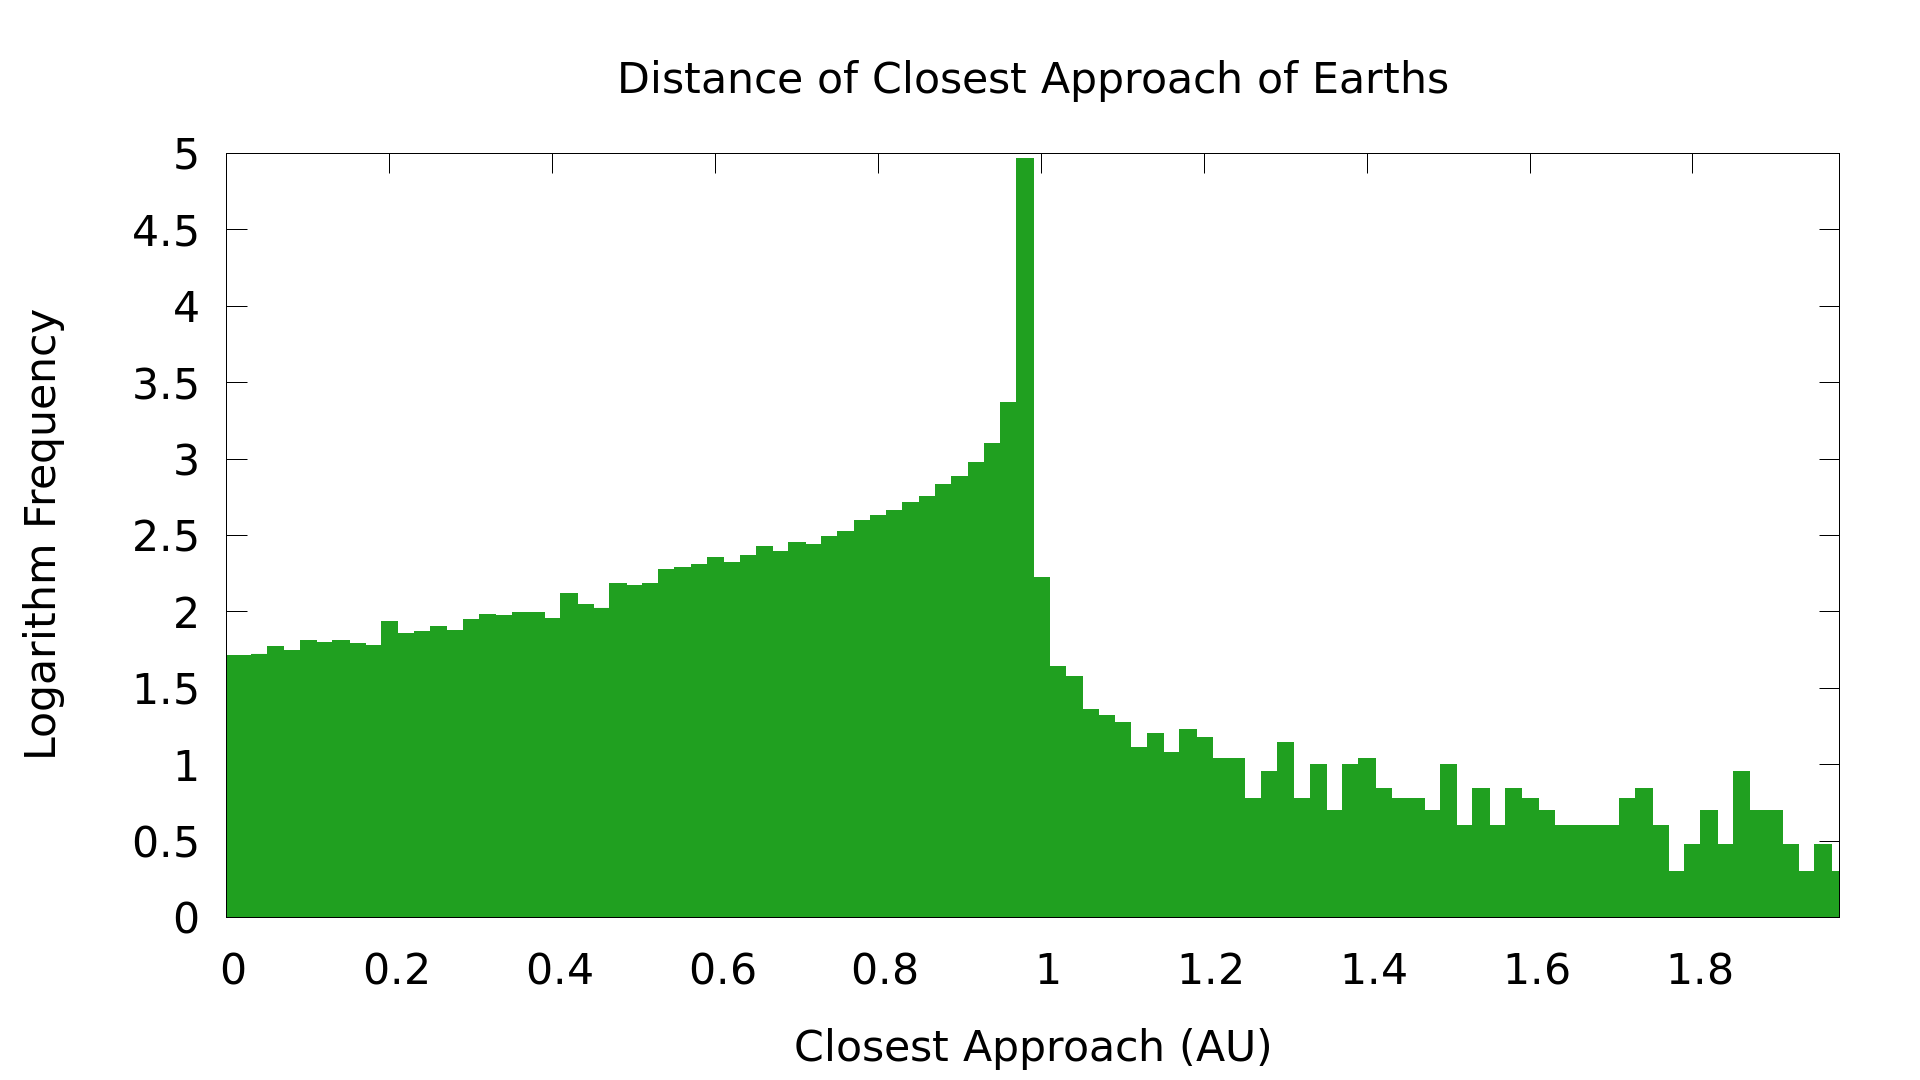
\includegraphics[width=3.25in]{periastron_earth_4000} &
            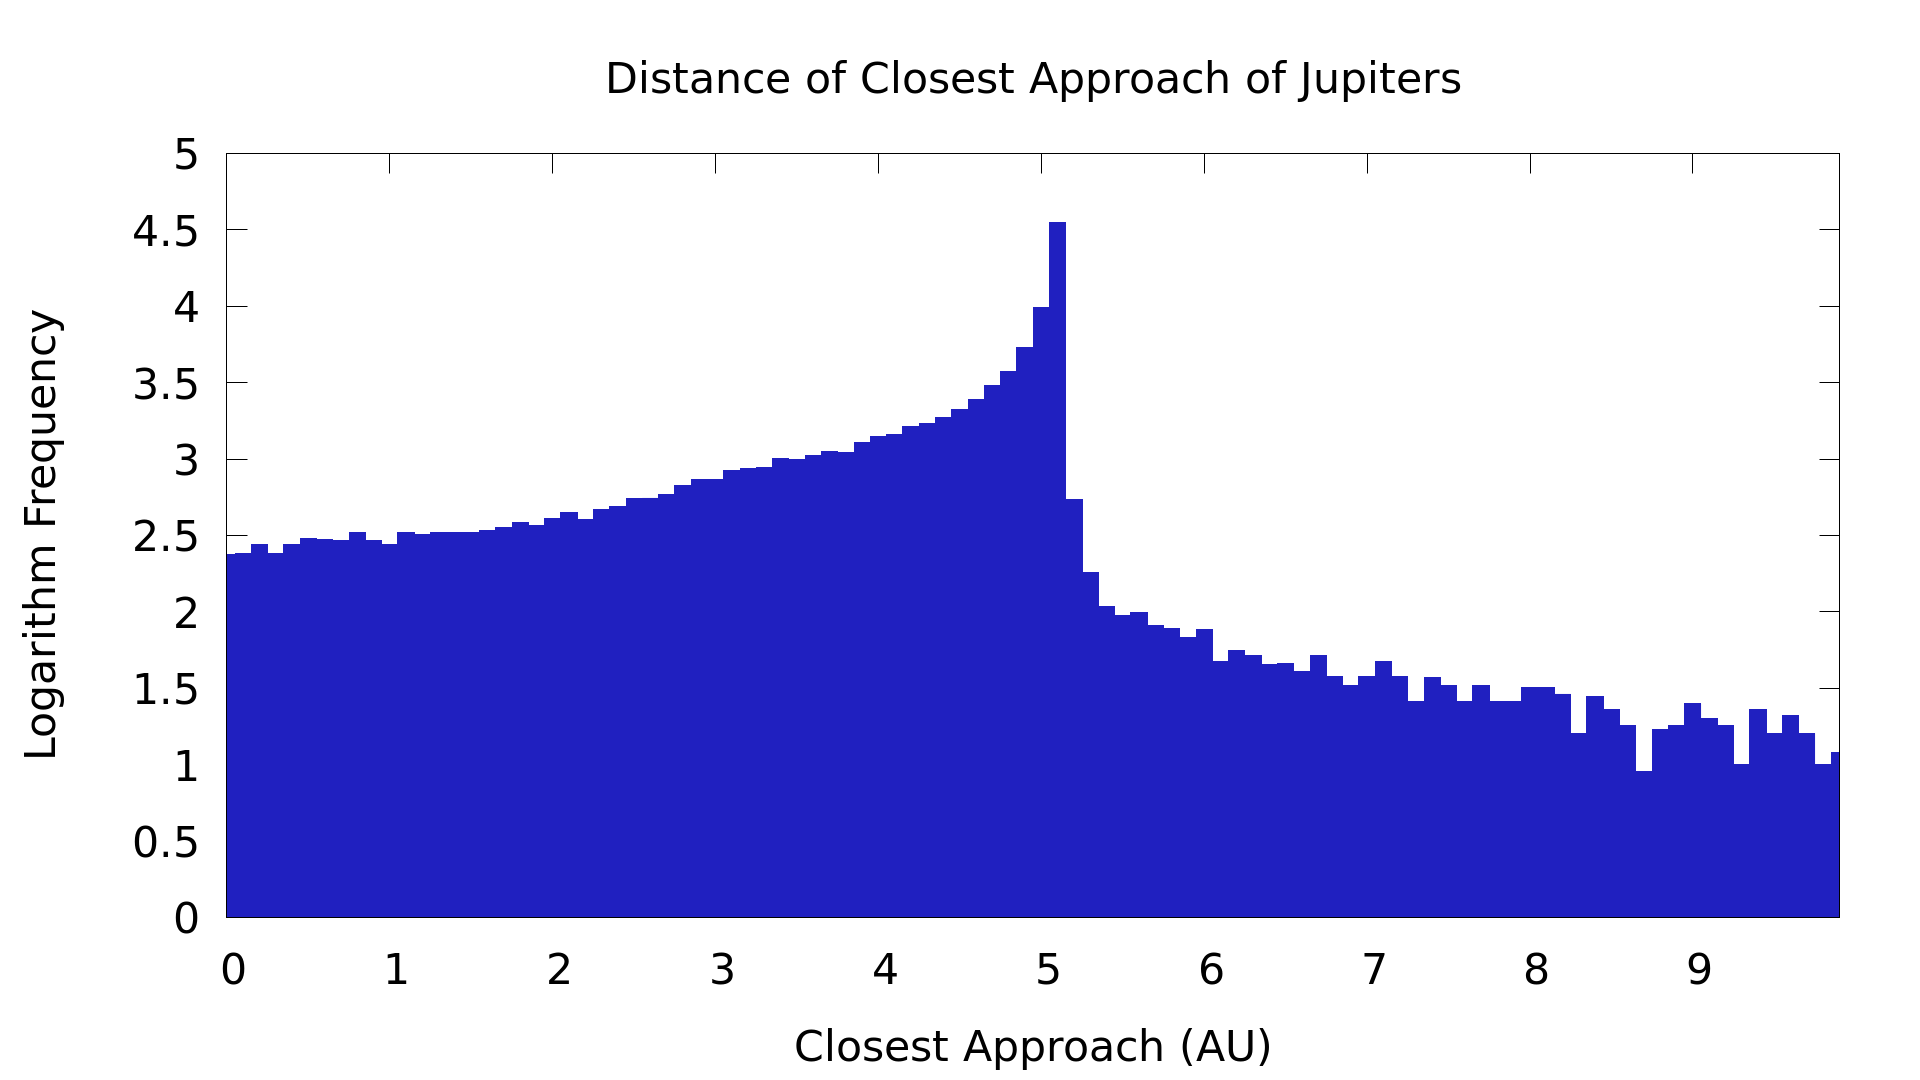
\includegraphics[width=3.25in]{periastron_jupiter_4000} \\
        \end{tabular}
    \end{figure}
    
    \begin{figure}[H]
        \centering
        \caption{Closest approach of Jupiter for 1000-star clusters, zoomed into the 
            closest 1 AU of the star.  The scale is linear.
        }

        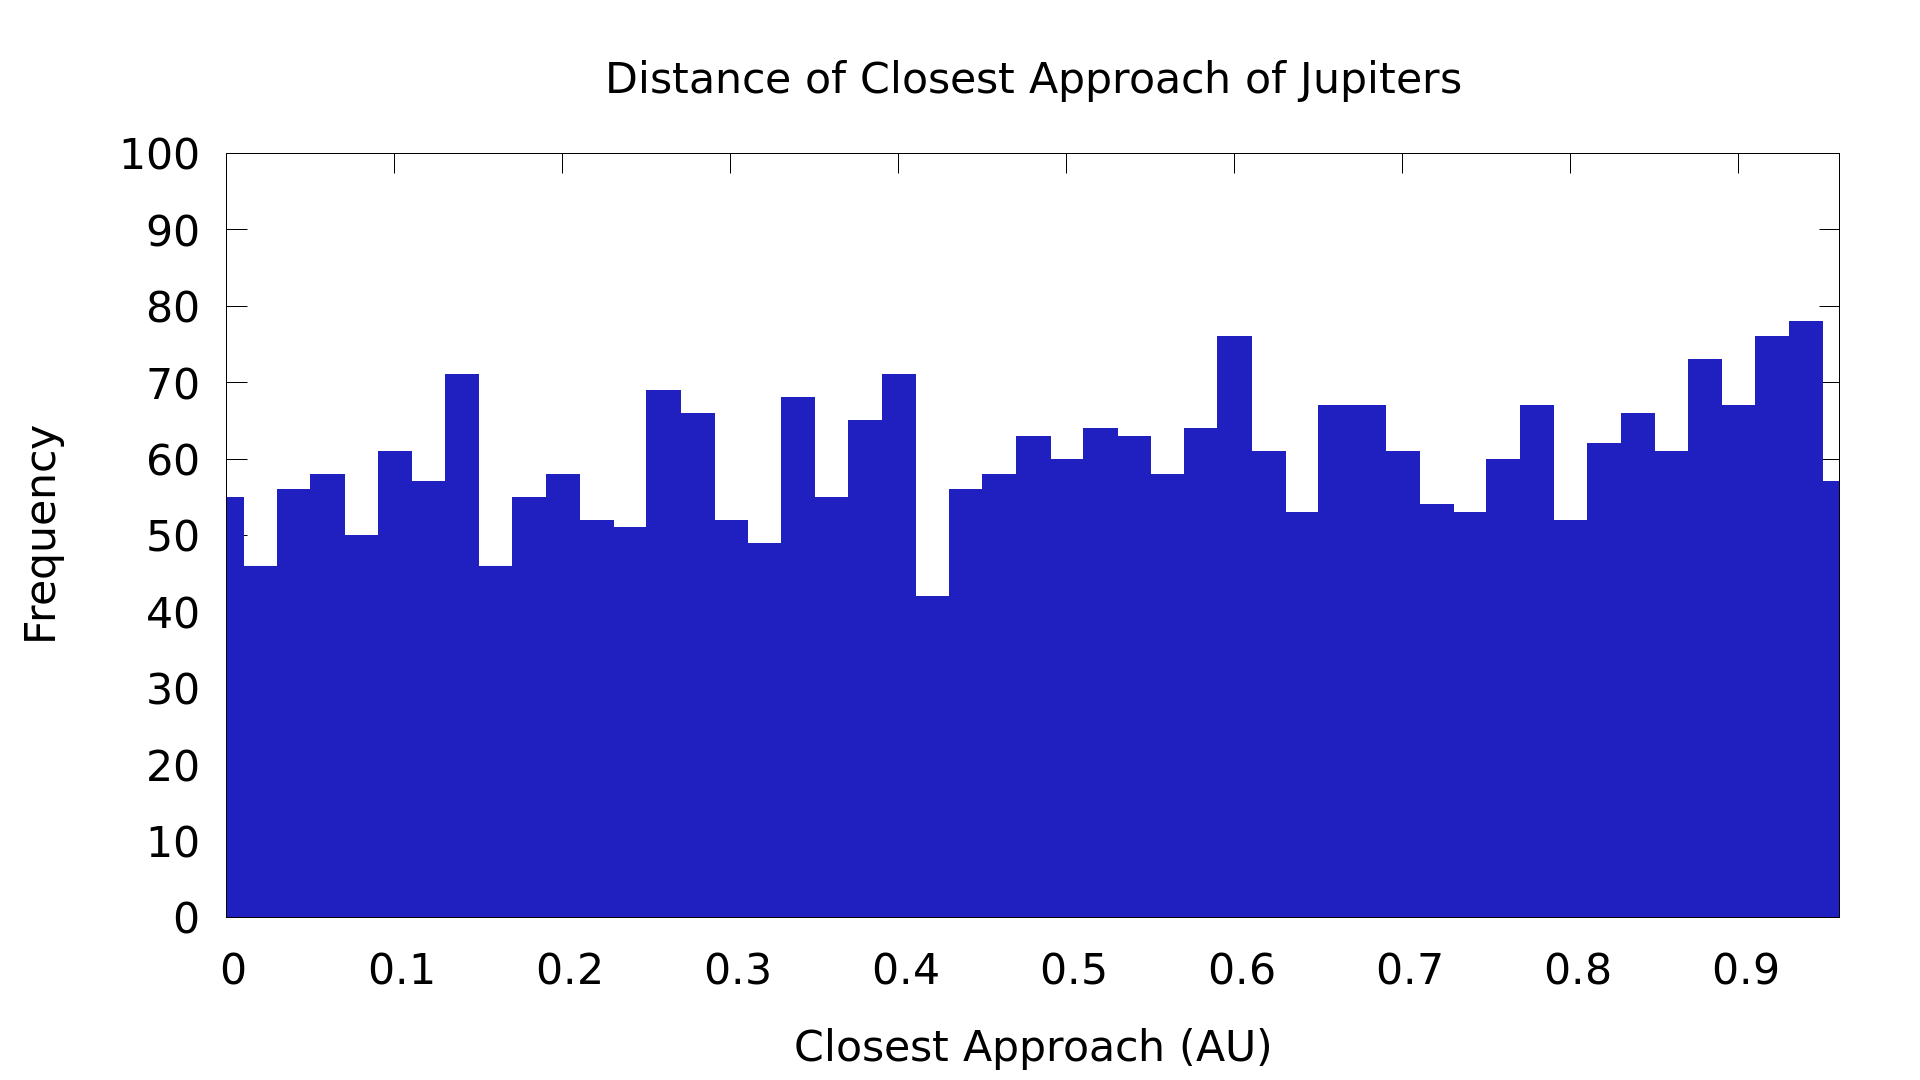
\includegraphics[width=3.25in]{periastron_jupiter_1000_close}
    \end{figure}

    To determine how much of an effect Jupiter migration had on the fate of the
    Earths, we plot the periastron of the two planet classes together. There is a
    very clear trend showing that relatively few Earths are perturbed significantly
    when the corresponding Jupiter is not perturbed significantly. However, once the 
    Jupiter migrates to within less than about two AU of the star, the corresponding Earth
    has a much larger chance to be perturbed. Furthermore, there is a clear trend
    showing that as the Jupiter periastron gets closer to the star, on average, so does
    the periastron of the Earth. By the time Jupiter comes closer than 1 AU 
    from the star, the Earth rarely survives unharmed.

    Interestingly, as the mass of the cluster increases, the Earths appear to be
    less strongly affected by the Jupiter migration. Figure \ref{fig:periastron}
    shows that the average frequency of close Jupiters does not significantly decrease
    in these more massive clusters, while the frequency of close Earths decreases
    by as much as half an order of magnitude in the closest cases.

    \begin{figure}[H]
        \caption{Periastron of Earth vs Jupiter for all encounters
            in each cluster group where neither planet escaped. From the top,
            the plots are for 1000-, 2000- and 4000-star clusters.
        }
        \centering
        \label{fig:evj_peri}
        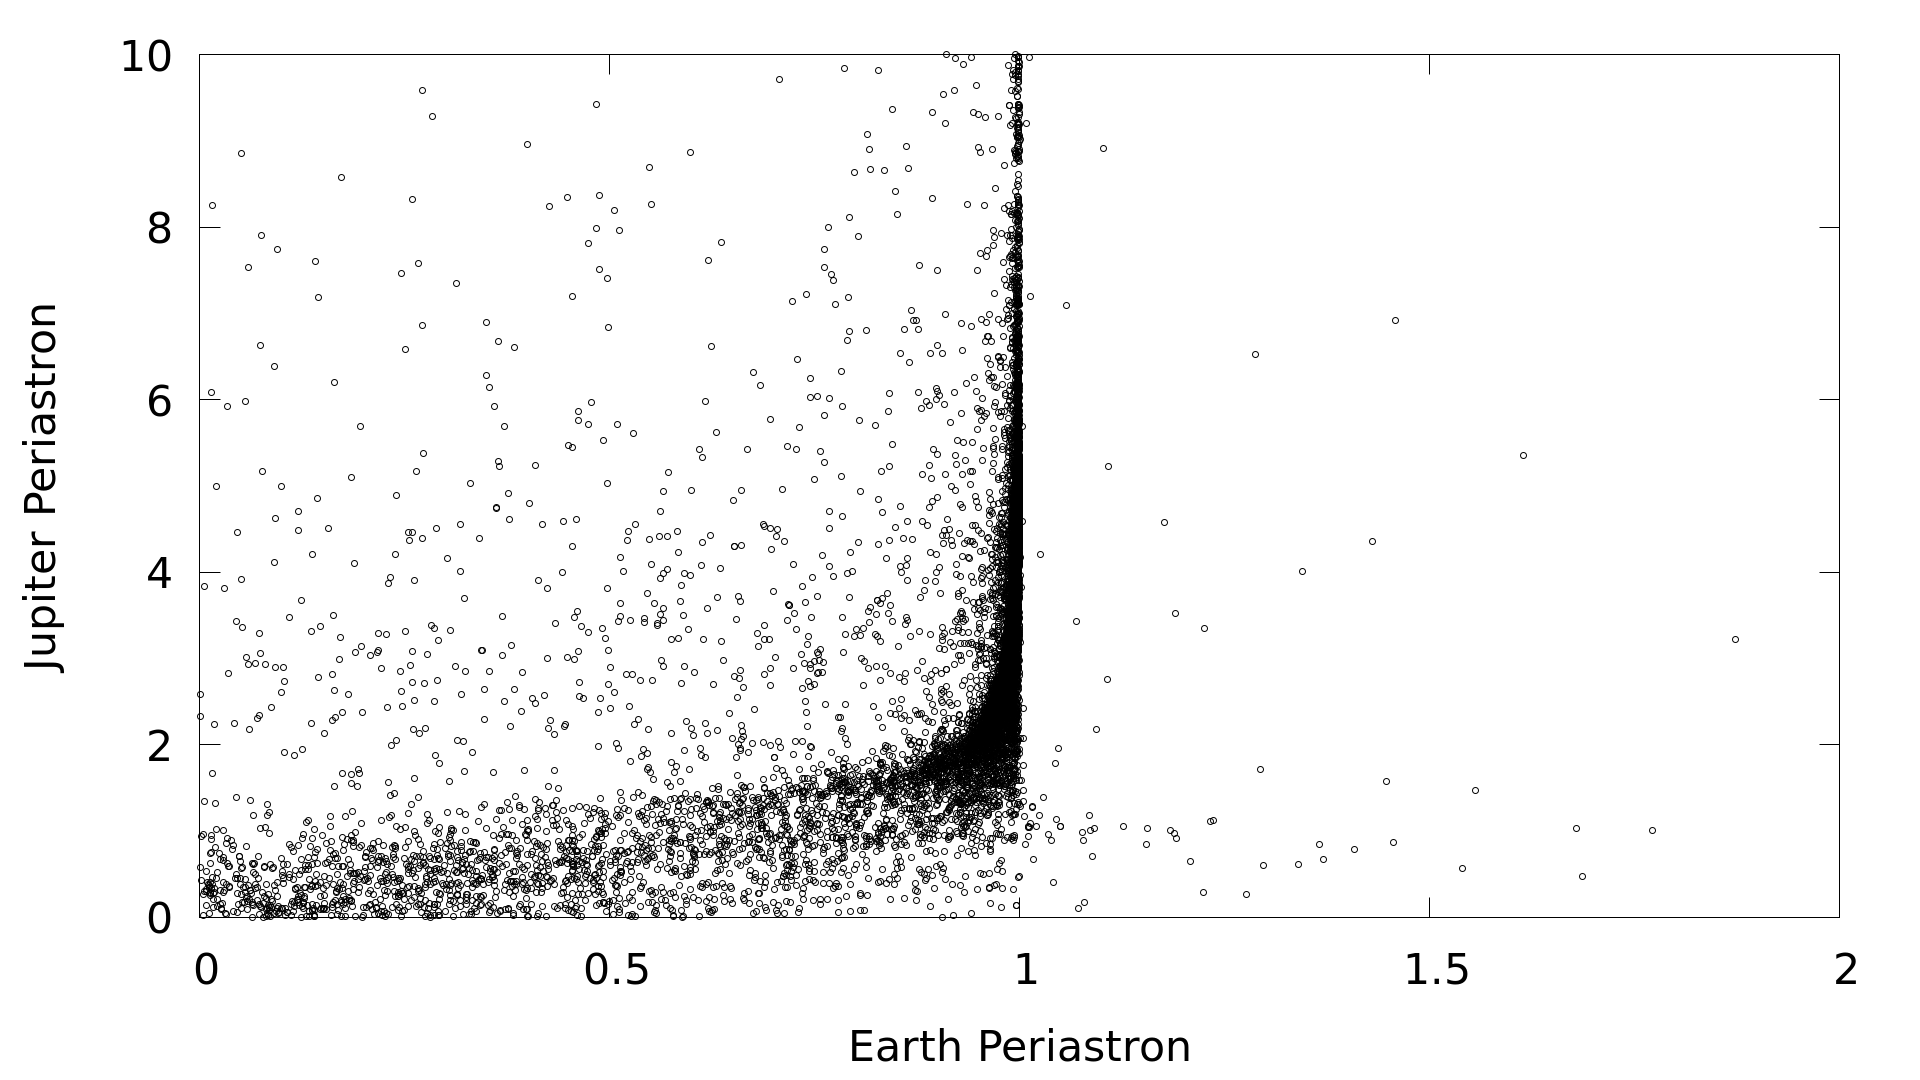
\includegraphics[width=5in]{evj_peri_earth_jupiter_1000} 
        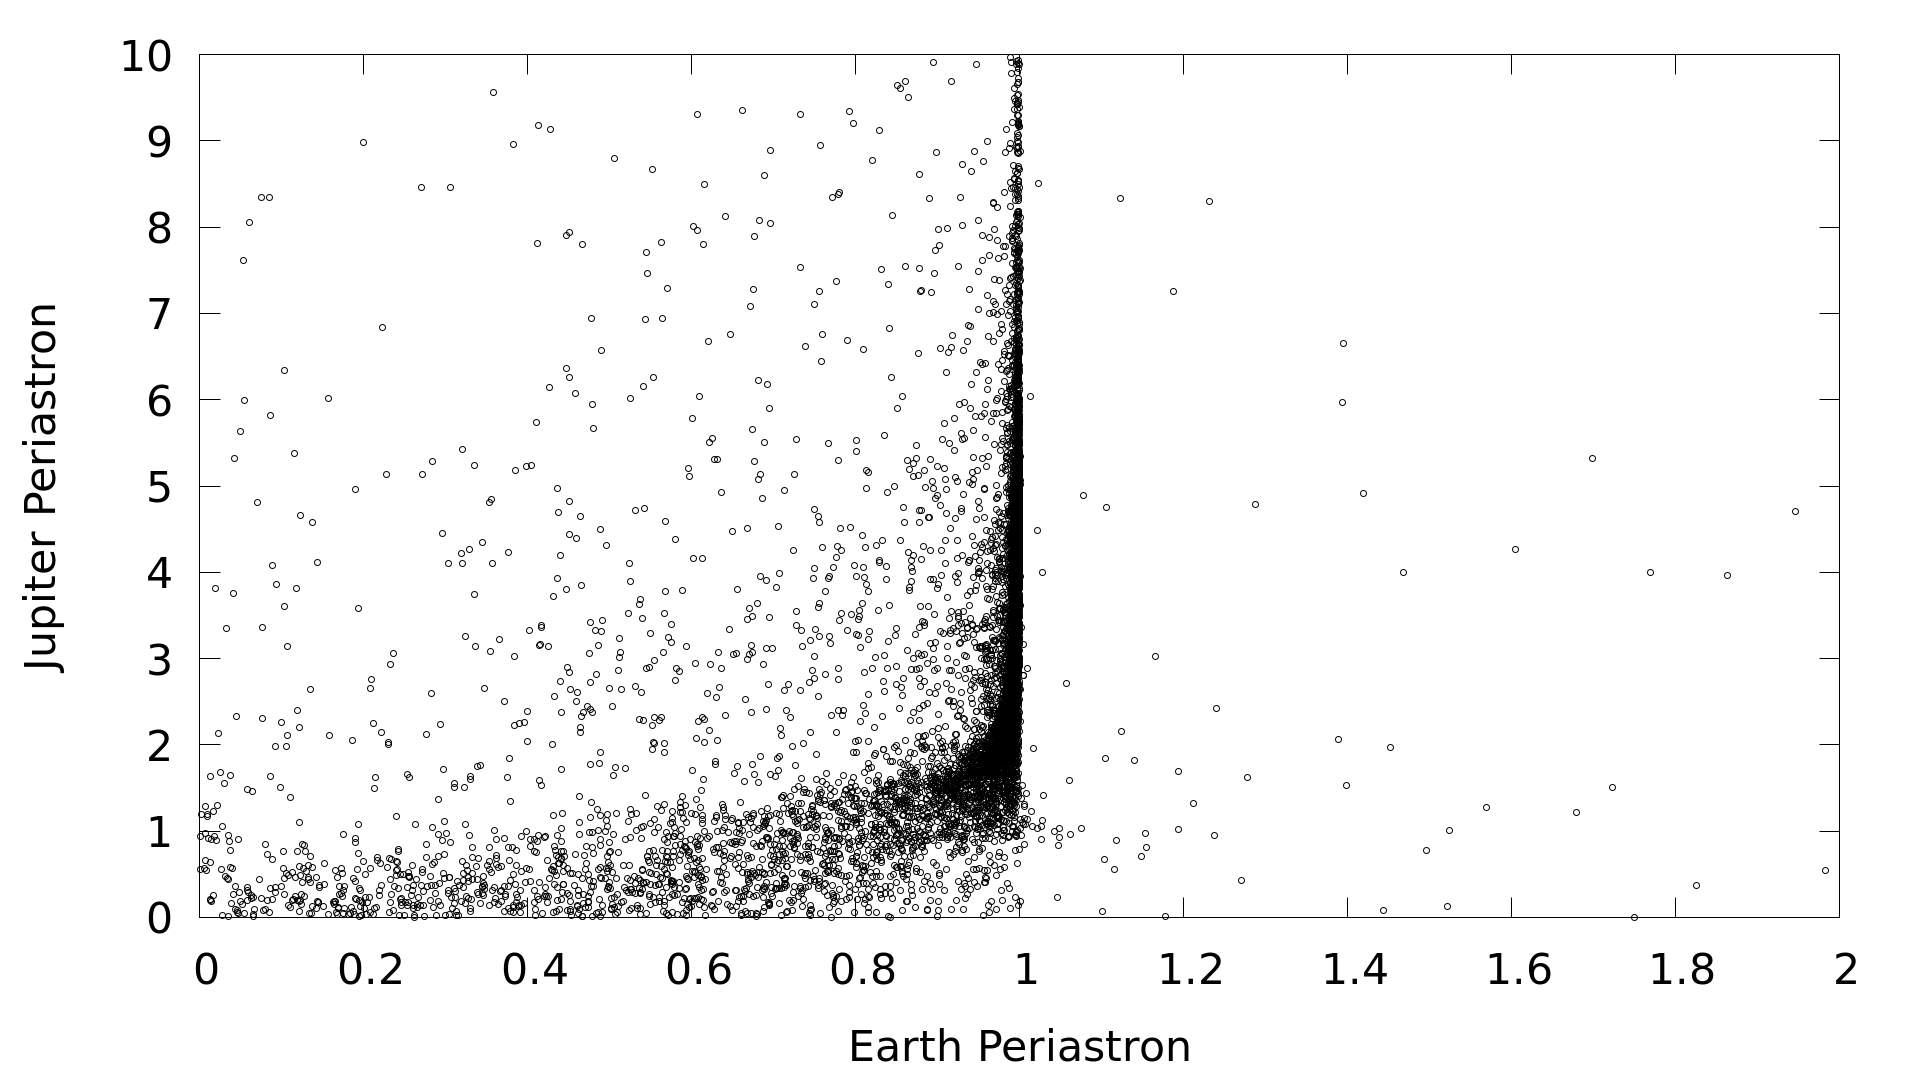
\includegraphics[width=5in]{evj_peri_earth_jupiter_2000} 
        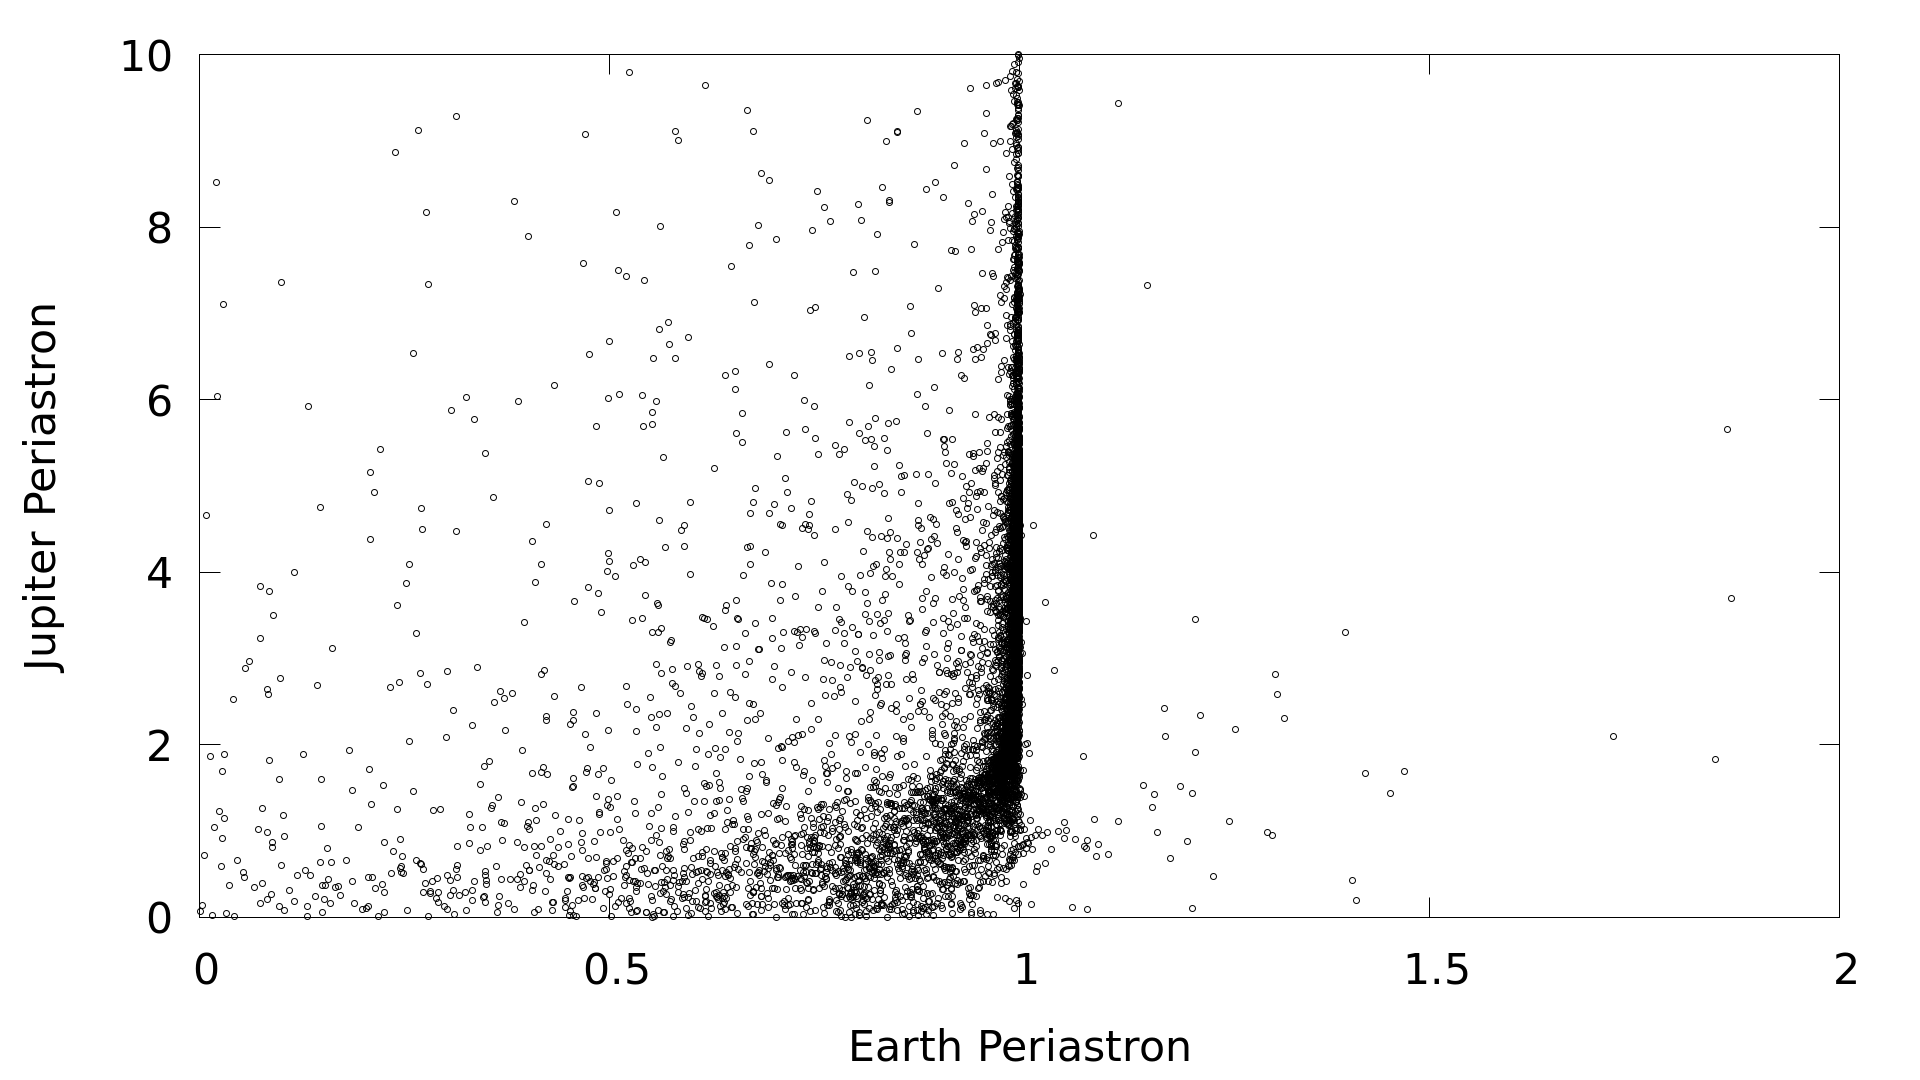
\includegraphics[width=5in]{evj_peri_earth_jupiter_4000} 
    \end{figure}

    Looking at the correlation of eccentricities of the final Earth
    and Jupiter systems, we see similar trends. In the 1000-star clusters,
    more high eccentricity Earths are in systems with high eccentricity Jupiters.
    Additionally, there appears to be a "bulge" around $e=0.5$ for the Jupiter
    where a large number of Earths are at least partially affected.

    Again, as with the periastron plots, we see many fewer high eccentricity
    Earths, though the general correlation between Earth and Jupiter periastron still
    exists.

    \begin{figure}[H]
        \caption{Eccentricity of Earth vs Jupiter for all encounters
            in each cluster group where neither planet escaped.The top
            plot is with 1000-star clusters while the bottom is with 4000-star
            clusters.
        }
        \centering
        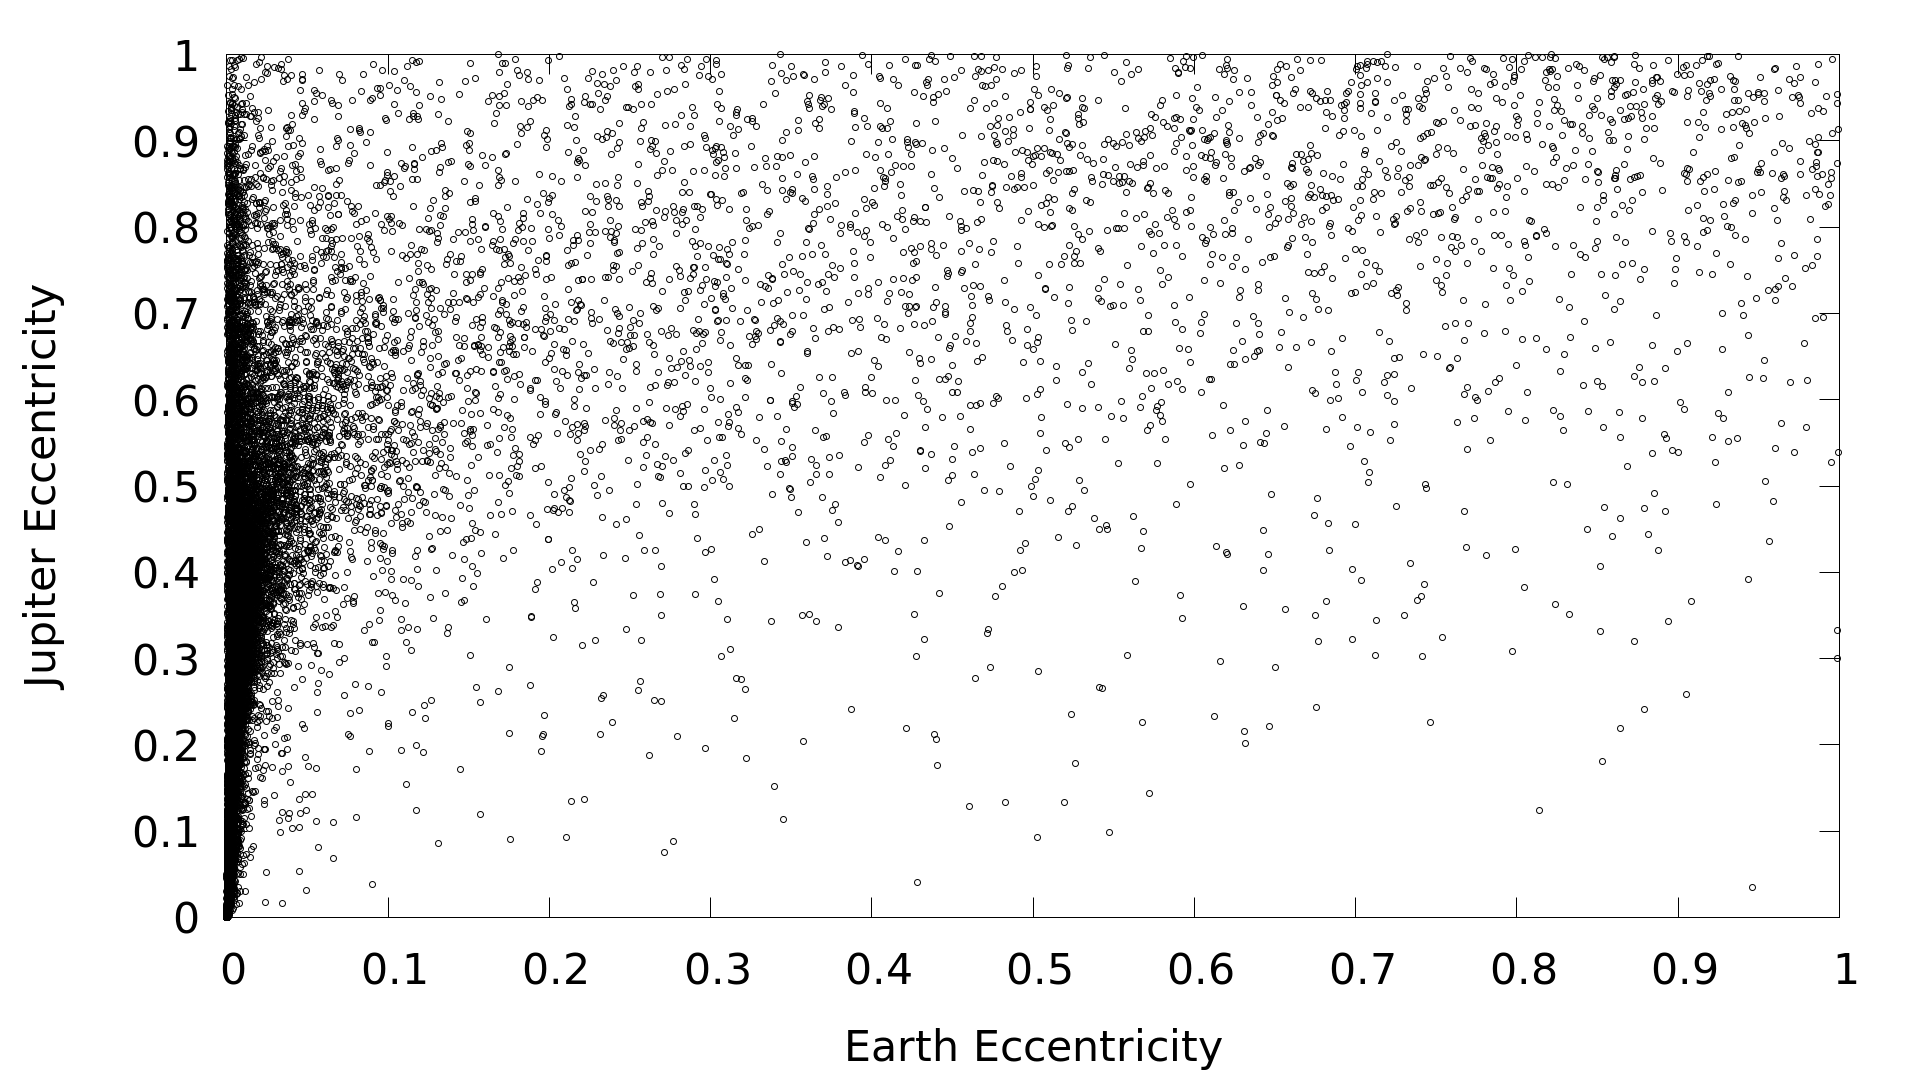
\includegraphics[width=5in]{evj_ecc_earth_jupiter_1000} 
        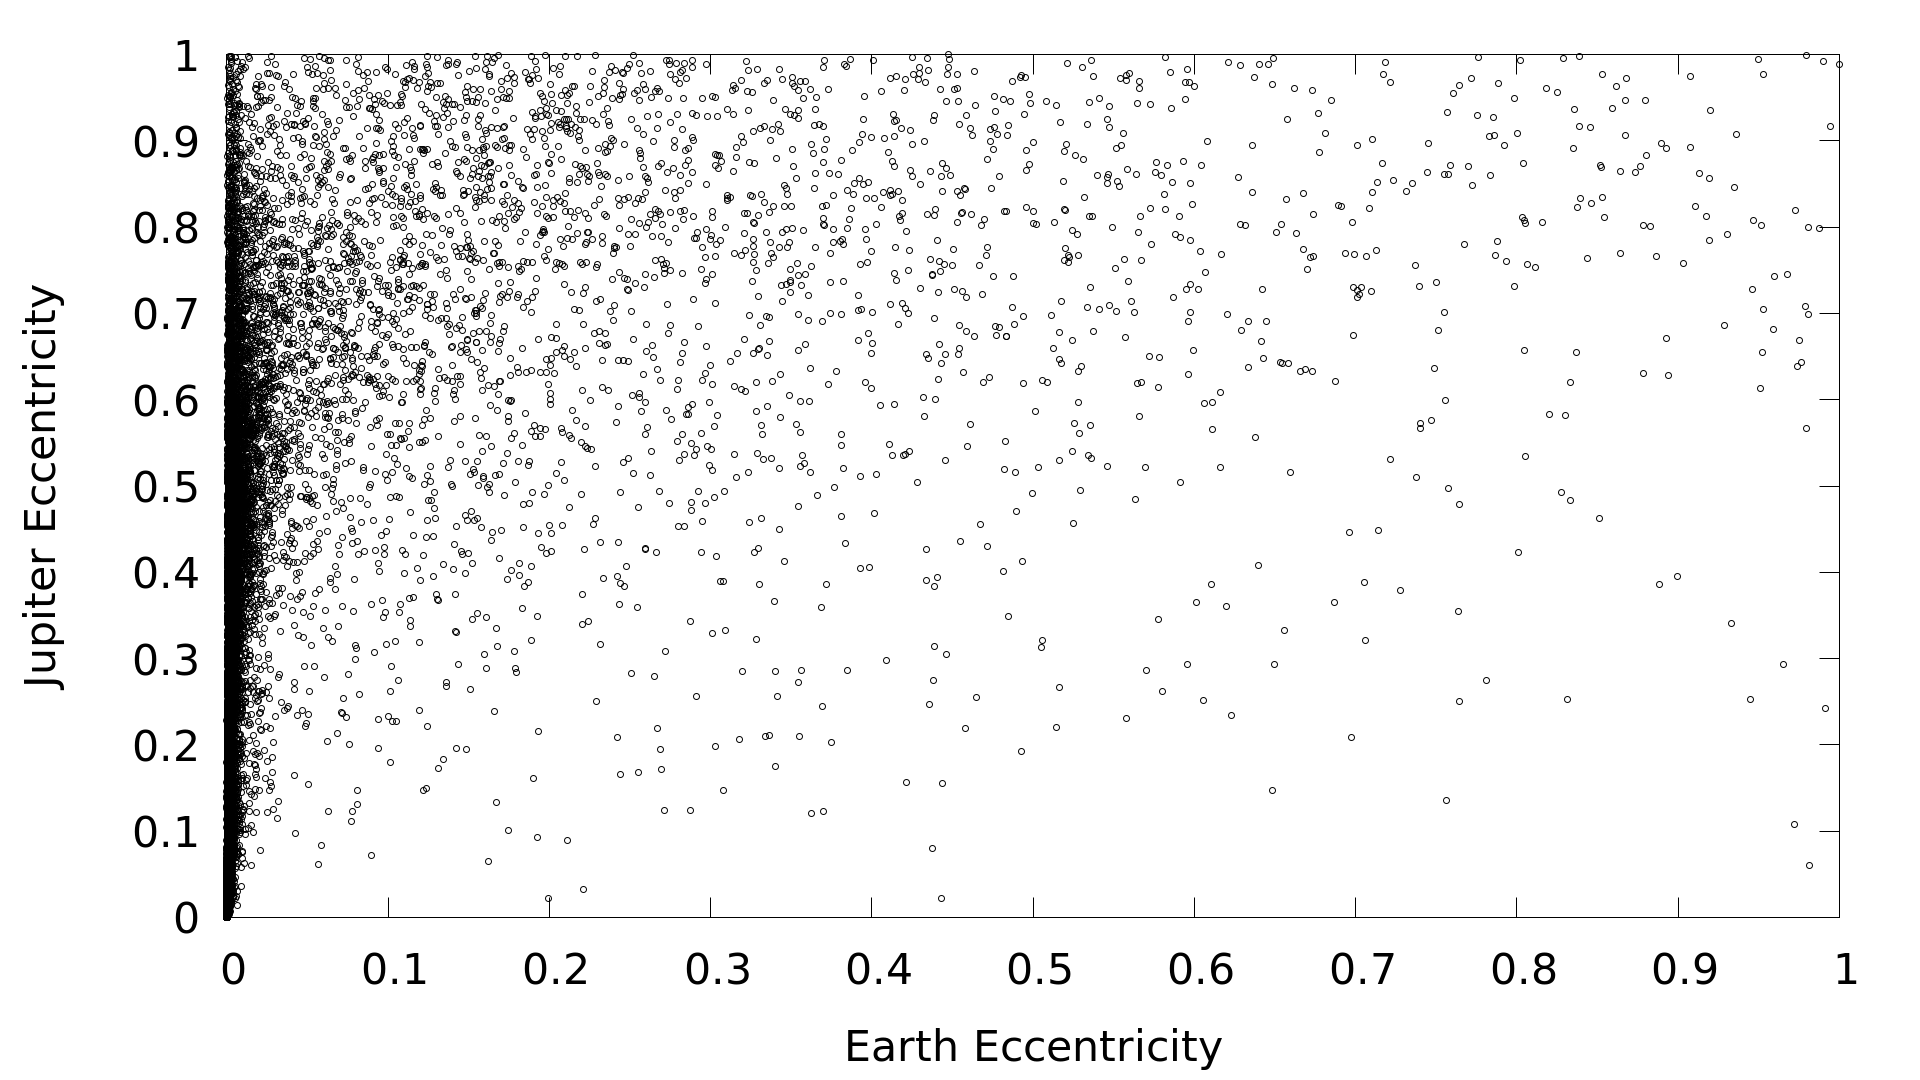
\includegraphics[width=5in]{evj_ecc_earth_jupiter_4000} 
    \end{figure}

    One final interesting analysis is to look at ejections and captures of planets.
    An ejection can be easily detected by searching for an $e \ge 1.0$ for a planet
    around both stars, whereas a capture can be detected by looking for $e \ge 1.0$ in
    the host star but $e < 1.0$ in the approaching star.

    We see over 10\% of all Jupiters are ejected, and around 2.5 \% of Earths are
    as well. Captures are a bit rarer, but they still occur with an appreciable
    frequency. The size of the cluster seems to have no effect on these statistics.

    \begin{table}[H]
        \centering
        \caption{Final states of Jupiter planets. Each row sums to 55,000.}
        \vspace{0.2in}
        \begin{tabular}{|llll|}
            \hline
            \textbf{Cluster Size} & \textbf{Remaining Planets} & \textbf{Ejected Planets} & \textbf{Captured Planets} \\
            \hline
            1000 & 46,935 & 6,472 & 1,593 \\
            2000 & 46,925 & 6,528 & 1,548 \\
            4000 & 47,146 & 6,343 & 1,511 \\
            \hline
        \end{tabular}
    \end{table}

    \begin{table}[H]
        \centering
        \caption{Final states of Earth planets. Each row sums to 55,000.}
        \vspace{0.2in}
        \begin{tabular}{|llll|}
            \hline
            \textbf{Cluster Size} & \textbf{Remaining Planets} & \textbf{Ejected Planets} & \textbf{Captured Planets} \\
            \hline
            1000 & 53,427 & 1,245 & 328 \\
            2000 & 53,489 & 1,229 & 282 \\
            4000 & 53,413 & 1,299 & 288 \\
            \hline
        \end{tabular}
    \end{table}

    %Future?

\section{Conclusion}

We explored a potential formation scenario for the formation of Hot Jupiter
planets using computational simulations to probe the physical universe. 
These planets have been observed in the universe with some frequency,
but their exact method of formation remains debated. 
We theorize that strong interactions between two planetary systems in a star
cluster could perturb the orbit of a normal gas giant to make it approach very close to
its host star. 

Our simulations show that this scenario is indeed a possibility, and that very close
interactions on the order of a few AU can frequently throw Jupiter-mass planets into
highly eccentric orbits with very close approaches to their host star. 
This may also drastically impact the orbits of other Earths 
in the system, with Jupiters migrating close to their host star being correlated
with Earths also being perturbed. This provides support for the idea that a Hot Jupiter may 
often have another pair planet that was thrown into an extreme orbit by the same
process that affected the Jupiter's orbit. Thus,
observation of these pair planets may provide reason to search for a Hot Jupiter
nearer the star.

Further long-term simulation will be needed to determine if the highly eccentric Jupiter
orbit could decay into a more circular orbit, similar to the many observed 
Hot Jupiters observed in our Galaxy, through tidal forces. Additional experiments may
also determine how more distantly orbiting planets such as Neptunes differ from Jupiter
in their behavior and whether they are more likely to form Hot Jupiters.

\clearpage

\begin{thebibliography}{9}

\bibitem{Pollack et al. 1996}
James B. Pollack, Olenka Hubickyj, Peter Bodenheimer, Jack J. Lissauer, Morris Podolak, Yuval Greenzweig, Formation of the Giant Planets by Concurrent Accretion of Solids and Gas, Icarus, Volume 124, Issue 1, 1996, Pages 62-85, ISSN 0019-1035, http://dx.doi.org/10.1006/icar.1996.0190.
(http://www.sciencedirect.com/science/article/pii/S0019103596901906)

\bibitem{Brucalassi, 2016}
A.  Brucalassi, L.  Pasquini, R.  Saglia, M. T.  Ruiz, P.  Bonifacio, I.  Leão, B. L.  Canto Martins, J. R.  de Medeiros, L. R.  Bedin, K.  Biazzo, C.  Melo, C.  Lovis, S.  Randich,
Search for giant planets in M67 - III. Excess of hot Jupiters in dense open clusters
A\&A 592 L1 (2016)
DOI: 10.1051/0004-6361/201527561

\bibitem{Foreman-Mackey et al. 2016}
Foreman-Mackey, D., Morton, T.~D., Hogg, D.~W., Agol, E., \& Sch{\"o}lkopf, B.\ 2016, arXiv:1607.08237 

\bibitem{Shara et al. 2014} Shara, M.~M., Hurley, J.~R., \& Mardling, R.~A.\ 2014, arXiv:1411.7061 

%	"HopInterface"
\bibitem{Eisenstein, Hut} Eisenstein, DJ, Hut, P, HOP: A new group-finding algorithm for N-body simulations, ApJ 498 (1998)
% "AMUSE"
\bibitem{Portegies Zwart} Portegies Zwart, S. et al., 2013, Multi-physics Simulations Using a Hierarchical Interchangeable Software Interface, Computer Physics Communications 183, 456-468 [2013CoPhC.183..456P]
		
\bibitem{Pelupessy et al. 2013} Pelupessy, F. I. et al., 2013, The Astrophysical Multipurpose Software Environment, Astronomy and Astrophysics 557, 84 [2013A\&A...557A..84P]
\bibitem{Portegis et al. 2009} Portegies Zwart, S. et al., 2009, A multiphysics and multiscale software environment for modeling astrophysical systems, *New Astronomy*, **Volume 14**, **Issue 4**, 369-378 [2009NewA...14..369P]

\bibitem{Rasiom et al. 1996} 
  F.~A.~Rasio, C.~A.~Tout, S.~H.~Lubow and M.~Livio,
  ``Tidal decay of close planetary orbits,''
  Astrophys.\ J.\  {\bf 470}, 1187 (1996)
  doi:10.1086/177941
  [astro-ph/9605059].
  %%CITATION = doi:10.1086/177941;%%
  %140 citations counted in INSPIRE as of 30 May 2017

\bibitem{King 1966} King, I.~R. 1966, "The structure of star clusters. III. Some simple dynamical models", The Astronomical Journal 71, 64 
doi:10.1086/109857
(http://adsabs.harvard.edu/abs/1966AJ.....71...64K)

\end{thebibliography}

\end{document}
